% OrderBookViz - Mini Project Report
% Build with XeLaTeX (run twice so the table of contents is complete):
%   xelatex OrderBookViz_Report.tex
% Code listings are read straight from the Java sources one folder up, so they
% always show the real code (line ranges refer to the current source files).

\documentclass[12pt,a4paper,openany,oneside]{report}

\usepackage[left=3cm,right=2.2cm,top=2.5cm,bottom=2.5cm,headheight=15pt]{geometry}
\usepackage{amsmath}
\usepackage{fontspec}
\IfFontExistsTF{Times New Roman}%
  {\setmainfont[Ligatures=TeX]{Times New Roman}}%
  {\IfFontExistsTF{TeX Gyre Termes}{\setmainfont[Ligatures=TeX]{TeX Gyre Termes}}{}}
\IfFontExistsTF{Menlo}%
  {\setmonofont[Scale=0.82]{Menlo}}%
  {\IfFontExistsTF{Courier New}%
    {\setmonofont[Scale=0.88]{Courier New}}%
    {\IfFontExistsTF{TeX Gyre Cursor}{\setmonofont{TeX Gyre Cursor}}{}}}

\usepackage{graphicx}
\usepackage{xcolor}
\usepackage{booktabs}
\usepackage{array}
\usepackage{longtable}
\usepackage{float}
\usepackage{caption}
\usepackage{subcaption}
\usepackage{setspace}
\usepackage{fancyhdr}
\usepackage{titlesec}
\usepackage{titletoc}
\usepackage{listings}
\usepackage{tikz}
\usetikzlibrary{shapes.multipart,shapes.geometric,positioning,arrows.meta,fit,backgrounds,calc}
\usepackage[hidelinks,pdftitle={OrderBookViz - Mini Project Report},pdfauthor={Parth Deshmukh, Sanket Kamboj}]{hyperref}

% ---------- editable cover-page details ----------
\newcommand{\projectTitle}{OrderBookViz}
\newcommand{\projectSubtitle}{A Java Swing Limit Order Book Simulator and Visualizer}
\newcommand{\guideName}{Dr. Jayendra Barua}
\newcommand{\guideDesignation}{Assistant Professor}

% ---------- small helpers ----------
\newcommand{\code}[1]{\texttt{#1}}
\newcolumntype{L}[1]{>{\raggedright\arraybackslash}p{#1}}
\newcommand{\keeplisting}[2][]{\lstinputlisting[float=htbp,#1]{#2}}
\renewcommand{\arraystretch}{1.25}
\setlength{\parindent}{0pt}
\setlength{\parskip}{6pt}
\setstretch{1.2}
\setcounter{tocdepth}{2}
\setcounter{secnumdepth}{3}
\renewcommand{\contentsname}{Table of Contents}

\captionsetup{font=small,labelfont=bf,skip=6pt}
\captionsetup[table]{position=above,skip=6pt}

% ---------- headings ----------
\titleformat{\chapter}[hang]{\normalfont\bfseries\fontsize{20}{24}\selectfont}{Chapter \thechapter:}{0.5em}{}
\titleformat{name=\chapter,numberless}[hang]{\normalfont\bfseries\fontsize{20}{24}\selectfont}{}{0pt}{}
\titlespacing*{\chapter}{0pt}{-14pt}{22pt}
\titleformat{\section}{\normalfont\Large\bfseries}{\thesection}{0.6em}{}
\titleformat{\subsection}{\normalfont\large\bfseries}{\thesubsection}{0.6em}{}
\titleformat{\subsubsection}{\normalfont\normalsize\bfseries}{\thesubsubsection}{0.6em}{}
\titlespacing*{\section}{0pt}{16pt}{6pt}
\titlespacing*{\subsection}{0pt}{12pt}{4pt}

% ---------- table of contents layout ----------
\titlecontents{chapter}[0em]{\addvspace{8pt}\bfseries}{Chapter \thecontentslabel:\quad}{}{\hfill\contentspage}
\titlecontents{section}[4.2em]{}{\contentslabel{2.6em}}{}{\titlerule*[0.5pc]{.}\contentspage}
\titlecontents{subsection}[7.8em]{}{\contentslabel{3.6em}}{}{\titlerule*[0.5pc]{.}\contentspage}

% ---------- header and footer ----------
\pagestyle{fancy}
\fancyhf{}
\fancyhead[L]{\small\projectTitle{} -- Mini Project Report}
\fancyhead[R]{\small\nouppercase{\leftmark}}
\fancyfoot[C]{\thepage}
\renewcommand{\headrulewidth}{0.4pt}
\fancypagestyle{plain}{\fancyhf{}\fancyfoot[C]{\thepage}\renewcommand{\headrulewidth}{0pt}}

% ---------- code listings ----------
\lstdefinestyle{java}{
  language=Java,
  basicstyle=\setstretch{1}\ttfamily\footnotesize,
  keywordstyle=\color{blue!60!black}\bfseries,
  commentstyle=\color{green!35!black}\itshape,
  stringstyle=\color{red!60!black},
  numbers=left, numberstyle=\tiny\color{gray}, numbersep=7pt,
  frame=single, rulecolor=\color{black!25}, backgroundcolor=\color{gray!5},
  breaklines=true, showstringspaces=false, tabsize=4,
  xleftmargin=1.6em, aboveskip=8pt, belowskip=4pt, captionpos=b
}
\lstset{style=java}
\lstdefinestyle{plain}{language={},numbers=none,xleftmargin=0pt,frame=single,
  basicstyle=\setstretch{1}\ttfamily\footnotesize,backgroundcolor=\color{gray!5},
  rulecolor=\color{black!25},aboveskip=6pt,belowskip=4pt}

% ---------- TikZ styles shared by the diagrams ----------
\tikzset{
  flow/.style={-{Latex[length=2.2mm]},thick},
  comp/.style={rectangle,draw,rounded corners=3pt,fill=white,align=center,
               minimum height=1.0cm,minimum width=3.9cm,inner sep=3pt},
  layerbox/.style={rectangle,draw=black!55,rounded corners=6pt,inner sep=9pt},
  lab/.style={font=\scriptsize,fill=white,inner sep=1.5pt},
  uc/.style={ellipse,draw,fill=blue!5,align=center,minimum width=4.4cm,
             minimum height=1.05cm,inner sep=1pt},
  act/.style={rectangle,rounded corners=6pt,draw,align=center,font=\footnotesize,
              fill=blue!6,minimum height=0.8cm,text width=4.4cm,inner sep=3pt},
  dec/.style={diamond,aspect=2.7,draw,align=center,font=\footnotesize,
              fill=yellow!14,inner sep=0pt,text width=3.2cm},
  st/.style={circle,fill=black,minimum size=0.35cm,inner sep=0pt},
  en/.style={circle,draw,thick,minimum size=0.5cm,inner sep=0pt,
             path picture={\fill (path picture bounding box.center) circle (0.14cm);}},
  badge/.style={circle,fill=red!75!black,text=white,font=\footnotesize\bfseries,
                minimum size=0.55cm,inner sep=0pt},
  cls/.style={rectangle split,rectangle split parts=3,draw,fill=white,font=\scriptsize,
              align=left,inner sep=3pt,text width=3.45cm,
              rectangle split part fill={blue!10,white,white}},
}

\begin{document}

% =====================================================================
%  COVER PAGE
% =====================================================================
\begin{titlepage}
\thispagestyle{empty}
\centering
\setstretch{1.0}

\includegraphics[height=2.9cm]{figures/thapar_logo.jpeg}\par
\vspace{0.5cm}
{\fontsize{22}{26}\selectfont\bfseries UCS553: Enterprise Web Application\par
 Mini Project Report\par}
\vspace{0.8cm}
{\fontsize{21}{25}\selectfont\bfseries \projectTitle\par}
\vspace{0.1cm}
{\large\bfseries \projectSubtitle\par}
\vspace{0.8cm}
{\Large Under the Guidance of\par}
\vspace{0.2cm}
{\Large\bfseries \guideName\par}
{\Large \guideDesignation\par}
{\Large Thapar Institute of Engineering \& Technology\par}
\vspace{0.8cm}
{\Large\bfseries Submitted By:\par}
\vspace{0.2cm}
{\Large
\begin{tabular}{@{}ll@{}}
1024031045 \hspace{1.2cm} & Parth Deshmukh\\
1024031042 \hspace{1.2cm} & Sanket Kamboj\\
\end{tabular}\par}
\vfill
{\large Computer Science \& Engineering Department\par
 Thapar Institute of Engineering \& Technology, Patiala\par}
\vspace{0.4cm}
{\normalsize In Partial Fulfilment of the Requirements for the Degree of\par
 Bachelor of Engineering in Computer Engineering\par
 at\par
 Thapar Institute of Engineering \& Technology, Patiala\par}
\vspace{0.5cm}
{\large\bfseries November 2026\par}
\end{titlepage}

% =====================================================================
%  ABSTRACT
% =====================================================================
\pagenumbering{roman}
\chapter*{Abstract}
\addcontentsline{toc}{chapter}{Abstract}
\markboth{Abstract}{Abstract}

Understanding how buy and sell orders meet in a financial market is difficult when the order book is only described in theory. \textbf{\projectTitle} is a Java Swing application that simulates a limit order book and draws it live, so that matching, liquidity, spread and price impact can be observed instead of imagined.

The heart of the system is an \code{OrderBook} that keeps bids (highest price first) and asks (lowest price first) in two \code{TreeMap} structures, matches every incoming limit order against the opposite side at the resting price, and rests whatever quantity is left over. A \code{MarketSimulator} drives three trading agents on a Swing timer: one market maker that quotes both sides of the mid price and two random traders. After every step the window shows a statistics row (best bid, best ask, spread, mid price and last trade), a line chart of the latest mid prices, the top ten bid and ask levels as depth bars, and the most recent trades.

The user can place their own limit orders, estimate the average fill price and price impact of a market order without changing the book, pause and resume the simulation, and change its speed. All input is validated: malformed numbers, out-of-range quantities and unrealistic prices are rejected through Java exception handling and reported as short messages instead of crashes.

The application needs nothing beyond the JDK, is organised into five source files of fewer than 700 lines in total, uses an object-oriented design with an abstract \code{Trader} hierarchy, and relies heavily on the Java Collections Framework. It is intended as an educational and prototyping tool and is not meant for live trading.

\textbf{Keywords:} limit order book, market microstructure, order matching, Java Swing, TreeMap, simulation, visualization.

% =====================================================================
%  TABLE OF CONTENTS
% =====================================================================
\tableofcontents

% =====================================================================
%  CHAPTER 1
% =====================================================================
\cleardoublepage
\pagenumbering{arabic}
\chapter{Introduction}

\section{Introduction to the Project}

Every modern exchange matches buyers and sellers with an electronic \emph{limit order book}. A limit order says ``buy (or sell) up to $N$ units at this price or better''. An order that cannot be matched immediately rests in the book: buy orders (\emph{bids}) are ranked from the highest to the lowest price and sell orders (\emph{asks}) from the lowest to the highest. The gap between the best bid and the best ask is the \emph{spread}, and their average is the \emph{mid price}. A new order priced at or beyond the best price on the opposite side is \emph{marketable}: it trades at once and consumes the resting liquidity level by level \cite{harris2003,gould2013}.

\textbf{\projectTitle} is a small desktop application that makes these ideas visible. It contains a matching engine, fills it with simulated traders, and draws the result in real time: a chart of the mid price, a ladder of the best bid and ask levels, the latest trades and a row of headline statistics. The user is not only a spectator. They can submit their own orders, ask what a large market order would do to the price, and pause or speed up the simulation.

The application is written in Java with the Swing toolkit \cite{swingtutorial} and uses nothing outside the standard JDK. Its five source files contain fewer than 700 lines of code, which keeps the whole design readable by a student in one sitting.

\section{Problem Statement}

Textbook explanations of order books rely on static tables. A learner cannot see how a single order consumes liquidity, how the spread widens when one side of the book is thin, or how quickly a market maker restores quotes after a large trade. Real exchange data feeds are binary, high-volume and often paid, and experimenting with real orders puts real money at risk. As a result, the mechanics of limit-order markets stay abstract for many students and developers.

\textbf{Problem statement:} \emph{to design and implement a self-contained Java desktop application that simulates a limit order book populated by automated market participants, visualizes the book and the price history in real time, and lets the user interact with the market safely.}

\section{Objectives of the Project}

\begin{enumerate}
  \item Implement a limit order book with price priority, using Java collections for the bid and ask sides.
  \item Implement a matching engine that fills marketable orders at the resting price, rests the remainder and records every trade.
  \item Simulate market participants as an object-oriented class hierarchy (a market maker and random traders) driven by a repeatable random generator.
  \item Visualize the mid price, the best bid and ask, the spread, the depth of the book and the latest trades live using Swing.
  \item Let the user place limit orders, estimate the impact of a market order without changing the book, pause or resume the simulation and change its speed.
  \item Validate every user input and handle errors with Java exceptions so that the program reports a clear message instead of failing.
  \item Keep the code simple and dependency-free so that it can be used for teaching and extended easily.
\end{enumerate}

\section{Scope of the Project}

\subsection*{Included in the scope}
\begin{itemize}
  \item A single instrument whose initial price is 100.0, with a price-priority order book that aggregates the quantity at each price level.
  \item Three simulated traders: one market maker (\code{MM-1}) and two random traders (\code{RT-1}, \code{RT-2}), driven by a random generator with a fixed seed so that every run is repeatable.
  \item Live visualization: statistics row, price chart (last 200 steps), depth ladder (top 10 levels per side) and a list of the 8 most recent trades.
  \item User interaction: placing limit orders, estimating market impact, pause and resume, and a speed control from 1 to 20 steps per second.
  \item Input validation and error reporting through exceptions.
\end{itemize}

\subsection*{Limitations}
\begin{itemize}
  \item Quantity is aggregated per price level, so \emph{time} priority between orders at the same price is not tracked; the engine implements price priority.
  \item Orders are never cancelled or expired, so resting liquidity accumulates during a long run.
  \item Trader \code{cash} and \code{inventory} are declared but not updated, because fills are not attributed to the resting counterparty.
  \item There is no self-trade prevention: a user order can match against a resting order placed earlier by the same user.
  \item Prices are \code{double} values shown with two decimals, so two levels that differ in the third decimal can look identical in the depth panel.
  \item Only limit orders can be placed; the effect of a market order is estimated, not executed.
  \item All state lives in memory and is lost when the window is closed.
\end{itemize}

\subsection*{Intended users}
Students learning data structures, trading systems or financial markets; developers prototyping order-book and market-simulation ideas; and instructors demonstrating matching engines and market depth. The tool is not meant for live trading or financial decision-making.

\subsection*{Future scope}
Order cancellation and expiry; owner-tracking orders so that profit and loss can be computed per trader; additional strategies such as momentum and mean-reversion traders; market and stop orders; exporting trades to CSV and replaying recorded order-book data; persistence with JDBC or SQLite; and a web front-end.

% =====================================================================
%  CHAPTER 2
% =====================================================================
\chapter{System Design}

\section{System Architecture}

\projectTitle{} is organised in three layers (Figure~\ref{fig:arch}). The \textbf{presentation layer} contains the Swing window and its two custom-painted panels. The \textbf{simulation layer} contains the simulator and the trading agents. The \textbf{core engine layer} contains the order book and the order value classes. Dependencies point downwards only: the engine knows nothing about traders or the GUI, and the simulation knows nothing about Swing.

\begin{figure}[htbp]
\centering
\resizebox{\linewidth}{!}{%
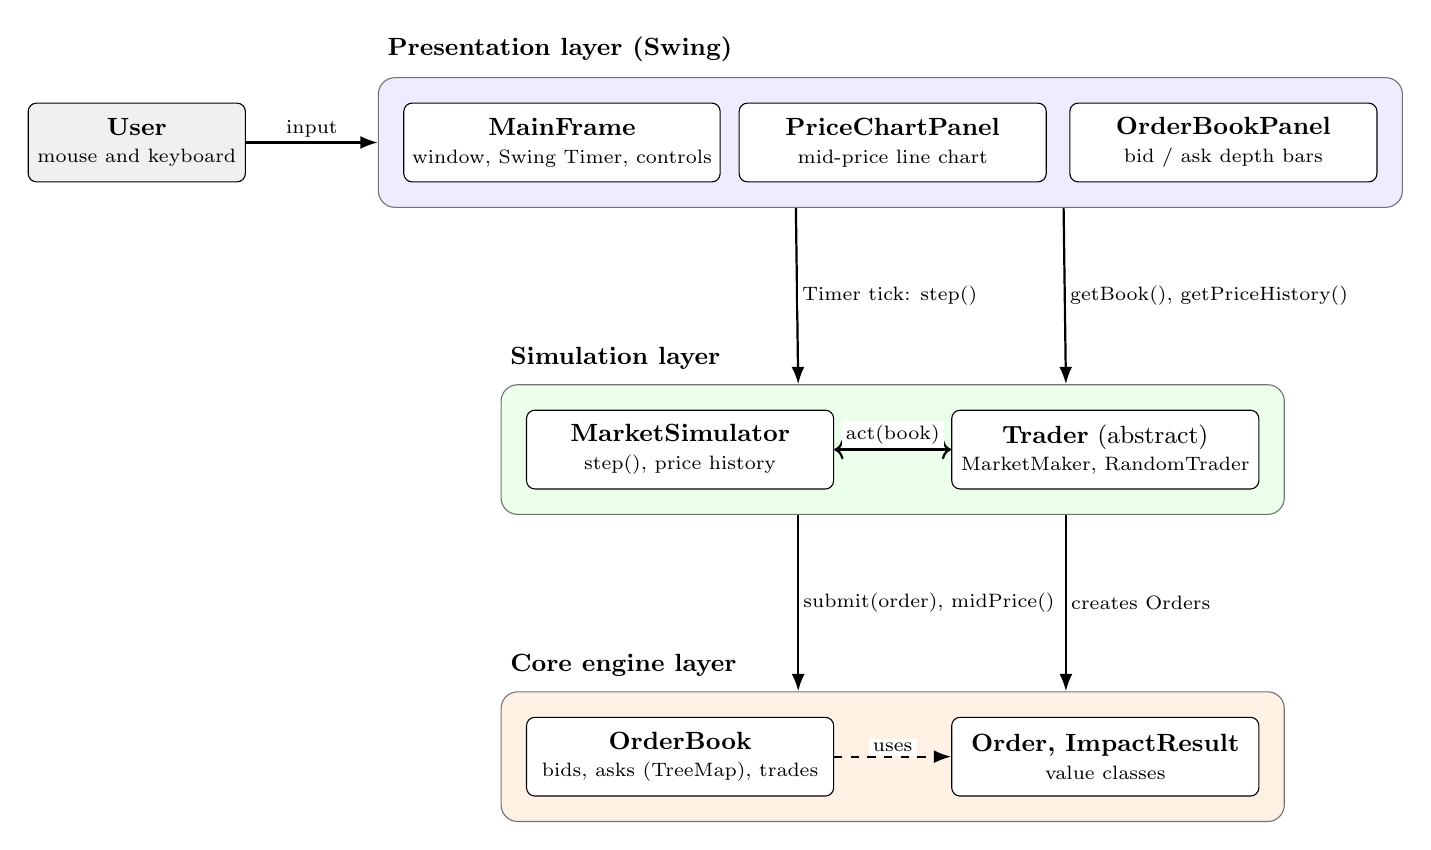
\begin{tikzpicture}[font=\small]
% presentation layer
\node[comp] (frame) at (-4.2,0) {\textbf{MainFrame}\\[-1pt]{\scriptsize window, Swing Timer, controls}};
\node[comp] (chart) at (0,0) {\textbf{PriceChartPanel}\\[-1pt]{\scriptsize mid-price line chart}};
\node[comp] (depth) at (4.2,0) {\textbf{OrderBookPanel}\\[-1pt]{\scriptsize bid / ask depth bars}};
\begin{scope}[on background layer]
 \node[layerbox,fill=blue!7,fit=(frame)(chart)(depth)] (L1) {};
\end{scope}
\node[anchor=south west,font=\small\bfseries] at ([yshift=2pt]L1.north west) {Presentation layer (Swing)};
% simulation layer
\node[comp] (sim) at (-2.7,-3.9) {\textbf{MarketSimulator}\\[-1pt]{\scriptsize step(), price history}};
\node[comp] (trd) at (2.7,-3.9) {\textbf{Trader} (abstract)\\[-1pt]{\scriptsize MarketMaker, RandomTrader}};
\begin{scope}[on background layer]
 \node[layerbox,fill=green!8,fit=(sim)(trd)] (L2) {};
\end{scope}
\node[anchor=south west,font=\small\bfseries] at ([yshift=2pt]L2.north west) {Simulation layer};
% core layer
\node[comp] (book) at (-2.7,-7.8) {\textbf{OrderBook}\\[-1pt]{\scriptsize bids, asks (TreeMap), trades}};
\node[comp] (ord) at (2.7,-7.8) {\textbf{Order, ImpactResult}\\[-1pt]{\scriptsize value classes}};
\begin{scope}[on background layer]
 \node[layerbox,fill=orange!10,fit=(book)(ord)] (L3) {};
\end{scope}
\node[anchor=south west,font=\small\bfseries] at ([yshift=2pt]L3.north west) {Core engine layer};
% flows
\draw[flow] ([xshift=-1.2cm]L1.south) -- node[lab,right]{Timer tick: step()} ([xshift=-1.2cm]L2.north);
\draw[flow] ([xshift=2.2cm]L1.south) -- node[lab,right]{getBook(), getPriceHistory()} ([xshift=2.2cm]L2.north);
\draw[flow,<->] (sim) -- node[lab,above]{act(book)} (trd);
\draw[flow] ([xshift=-1.2cm]L2.south) -- node[lab,right]{submit(order), midPrice()} ([xshift=-1.2cm]L3.north);
\draw[flow] ([xshift=2.2cm]L2.south) -- node[lab,right]{creates Orders} ([xshift=2.2cm]L3.north);
\draw[flow,dashed] (book) -- node[lab,above]{uses} (ord);
% user
\node[draw,rounded corners=3pt,fill=gray!12,align=center,minimum height=1.0cm] (user) at (-9.6,0) {\textbf{User}\\[-1pt]{\scriptsize mouse and keyboard}};
\draw[flow] (user) -- node[lab,above]{input} (L1.west);
\end{tikzpicture}}
\caption{Layered architecture of \projectTitle{}. Arrows show the direction of calls.}
\label{fig:arch}
\end{figure}

\subsection*{Data flow}
\begin{enumerate}
  \item A \code{javax.swing.Timer} fires on the Swing event thread every $1000/\text{speed}$ milliseconds (200~ms at the default speed of 5 steps per second) \cite{timerapi}.
  \item \code{MainFrame} calls \code{simulator.step()}.
  \item Each trader, in a fixed order, reads the book (\code{midPrice()}) and returns a list of orders.
  \item Every order is passed to \code{book.submit()}, which matches it against the opposite side, rests the remainder and records any trades.
  \item The simulator appends the new mid price to its history.
  \item \code{MainFrame.refresh()} updates the labels and the trade list and repaints the two panels, which read the book and the history directly.
\end{enumerate}
User actions follow a shorter path: \code{placeOrder()} validates the input and calls \code{book.submit()} with trader id \code{YOU}, while \code{estimateImpact()} calls the read-only \code{book.estimateImpact()}. Because the timer, the button handlers and the painting all run on the single Swing event thread, no locking is needed.

\section{Use Case Diagram}

The system has two actors: the \textbf{User} (a student or instructor) and the \textbf{Swing Timer}, a system actor that triggers every simulation step. Figure~\ref{fig:usecase} shows the use cases and Table~\ref{tab:usecases} describes them.

\begin{figure}[htbp]
\centering
\resizebox{\linewidth}{!}{%
\begin{tikzpicture}[font=\small,>={Latex[length=2.2mm]}]
\draw[rounded corners=8pt,fill=gray!5] (2.3,-8.2) rectangle (13.8,2.2);
\node[font=\bfseries] at (8.05,1.75) {\projectTitle};
% user actor
\begin{scope}[shift={(0.5,-3.4)}]
 \draw (0,0.95) circle (0.22);
 \draw (0,0.73)--(0,0.05)--(-0.3,-0.5);
 \draw (0,0.05)--(0.3,-0.5);
 \draw (-0.4,0.5)--(0.4,0.5);
 \node[below] at (0,-0.5) {User};
\end{scope}
% use cases
\node[uc] (u1) at (5.0,0.7) {View live price chart\\and statistics};
\node[uc] (u2) at (5.0,-0.9) {View order-book depth\\and recent trades};
\node[uc] (u3) at (5.0,-2.5) {Place limit order};
\node[uc] (u4) at (5.0,-4.1) {Estimate market impact};
\node[uc] (u5) at (5.0,-5.7) {Pause / resume simulation};
\node[uc] (u6) at (5.0,-7.3) {Adjust simulation speed};
\node[uc] (u7) at (11.2,0.7) {Advance simulation step};
\node[uc] (u8) at (11.2,-2.5) {Match orders};
\node[uc] (u9) at (11.2,-4.1) {Validate input};
% actor links
\foreach \u in {u1,u2,u3,u4,u5,u6}{\draw (0.5,-3.0) -- (\u.west);}
% system actor
\node[draw,rectangle,fill=gray!12,align=center,minimum height=1.0cm] (timer) at (15.4,0.7) {{\scriptsize\guillemotleft system\guillemotright}\\\textbf{Swing Timer}};
\draw (timer.west) -- (u7.east);
% includes
\draw[->,dashed] (u3) -- node[above,font=\scriptsize]{\guillemotleft include\guillemotright} (u8);
\draw[->,dashed] (u7) -- node[right,font=\scriptsize]{\guillemotleft include\guillemotright} (u8);
\draw[->,dashed] (u3.south east) -- node[above,font=\scriptsize,sloped,pos=0.4]{\guillemotleft include\guillemotright} (u9.north west);
\draw[->,dashed] (u4.east) -- node[above,font=\scriptsize]{\guillemotleft include\guillemotright} (u9.west);
\end{tikzpicture}}
\caption{Use case diagram of \projectTitle{}.}
\label{fig:usecase}
\end{figure}

\begin{table}[H]
\centering\small
\caption{Use cases of \projectTitle{}.}
\label{tab:usecases}
\begin{tabular}{@{}l L{4.1cm} L{2.4cm} L{6.4cm}@{}}
\toprule
\textbf{ID} & \textbf{Use case} & \textbf{Actor} & \textbf{Description}\\
\midrule
UC1 & View live price chart and statistics & User & Watch best bid, best ask, spread, mid price, last trade and the mid-price line chart.\\
UC2 & View order-book depth and recent trades & User & See the top 10 bid and ask levels as bars and the 8 latest trades.\\
UC3 & Place limit order & User & Submit a BUY or SELL order with a price and quantity; see how much filled and how much rests.\\
UC4 & Estimate market impact & User & Ask for the average fill price and price impact of a market order of a given size; the book is not changed.\\
UC5 & Pause / resume simulation & User & Stop or restart the Swing Timer.\\
UC6 & Adjust simulation speed & User & Choose 1 to 20 simulation steps per second.\\
UC7 & Advance simulation step & Swing Timer & Let every trader act once and record the new mid price.\\
UC8 & Match orders & (included) & Match an order against the opposite side and rest the remainder.\\
UC9 & Validate input & (included) & Reject malformed or out-of-range values with a message.\\
\bottomrule
\end{tabular}
\end{table}

\begin{table}[H]
\centering\small
\caption{Use case specification: UC3 -- Place limit order.}
\begin{tabular}{@{}L{3.1cm} L{11.9cm}@{}}
\toprule
\textbf{Actor} & User\\
\textbf{Precondition} & The application window is open (the simulation may be running or paused).\\
\textbf{Main flow} & 1.~The user selects BUY or SELL and types a price and a quantity.\newline
2.~The user clicks \emph{Place Order} or presses Enter in a field.\newline
3.~The system validates the input (UC9).\newline
4.~The system creates the order with trader id \code{YOU} and submits it to the book (UC8).\newline
5.~The system shows ``\emph{SIDE qty @ price: x filled, y resting}'' in green and refreshes all views.\\
\textbf{Alternate flow} & At step 3 the input is invalid: the system shows a red error message, the book is not changed and the user may correct the value.\\
\textbf{Postcondition} & The book contains the unfilled remainder (if any) at the chosen price; filled quantity appears in the trade list.\\
\bottomrule
\end{tabular}
\end{table}

\begin{table}[H]
\centering\small
\caption{Use case specification: UC4 -- Estimate market impact.}
\begin{tabular}{@{}L{3.1cm} L{11.9cm}@{}}
\toprule
\textbf{Actor} & User\\
\textbf{Precondition} & The application window is open.\\
\textbf{Main flow} & 1.~The user selects the side and types a quantity.\newline
2.~The user clicks \emph{Estimate Impact}.\newline
3.~The system validates the quantity and walks the opposite side of the book from the best price without changing it.\newline
4.~The system shows ``\emph{SIDE qty at market: filled=\ldots\ avg=\ldots\ impact=\ldots}''.\\
\textbf{Alternate flow} & The quantity is invalid: a red error message is shown.\\
\textbf{Postcondition} & The book, the trade list and the chart are unchanged.\\
\bottomrule
\end{tabular}
\end{table}

\section{Class Diagram}

Figure~\ref{fig:class} shows the classes of the system. \code{MarketMaker} and \code{RandomTrader} inherit from the abstract class \code{Trader}. \code{MainFrame} \emph{owns} its two panels and the simulator (composition), and the simulator owns the order book and aggregates its traders. The panels and the traders only \emph{use} the simulator or the book (dependency). \code{Trader.act()} returns \code{Order} objects and \code{MainFrame} also creates them for the user's orders; these dependencies are left out of the figure to keep it readable.

\begin{figure}[H]
\centering
\resizebox{0.98\linewidth}{!}{%
\begin{tikzpicture}[font=\small,>={Latex[length=2.4mm]}]
% row 1
\node[cls] (chartp) at (0,0) {{\centering\textbf{PriceChartPanel}\par}\textit{extends JPanel}
 \nodepart{second}-simulator: MarketSimulator\\-POINTS: int = 200
 \nodepart{third}\#paintComponent(Graphics)};
\node[cls,text width=4.1cm] (frame) at (6.9,0) {{\centering\textbf{MainFrame}\par}\textit{extends JFrame}
 \nodepart{second}-simulator: MarketSimulator\\-chart: PriceChartPanel\\-bookPanel: OrderBookPanel\\-timer: Timer
 \nodepart{third}+MainFrame()\\-placeOrder()\\-estimateImpact()\\-readPrice(): double\\-readQuantity(): int\\-togglePause()\\-changeSpeed()\\-refresh()\\+main(String[])};
\node[cls] (bookp) at (13.8,0) {{\centering\textbf{OrderBookPanel}\par}\textit{extends JPanel}
 \nodepart{second}-simulator: MarketSimulator\\-LEVELS: int = 10
 \nodepart{third}\#paintComponent(Graphics)\\-topLevels(Map)\\-drawLevels(...)};
% row 2
\node[cls,text width=4.1cm] (sim) at (6.9,-7.6) {{\centering\textbf{MarketSimulator}\par}
 \nodepart{second}-book: OrderBook\\-traders: List<Trader>\\-priceHistory: List<Double>
 \nodepart{third}+step()\\+getBook(): OrderBook\\+getPriceHistory(): List<Double>\\+getTraders(): List<Trader>};
% row 3
\node[cls] (trader) at (1.6,-13.2) {{\centering\textbf{Trader}\par}{\centering\textit{\guillemotleft abstract\guillemotright}\par}
 \nodepart{second}\#id: String\\\#cash: double\\\#inventory: int
 \nodepart{third}+act(OrderBook): List<Order>\\+getId(), getCash()\\+getInventory()};
\node[cls,text width=4.1cm] (ob) at (12.2,-13.2) {{\centering\textbf{OrderBook}\par}
 \nodepart{second}-bids: TreeMap<Double,Integer>\\-asks: TreeMap<Double,Integer>\\-trades: List<String>\\-lastPrice: double
 \nodepart{third}+submit(Order)\\-matchBuy(Order)\\-matchSell(Order)\\+bestBid(), bestAsk(): Double\\+midPrice(): double\\+estimateImpact(Side,int)\\+getBids(), getAsks()\\+getTrades(): List<String>};
% row 4
\node[cls] (mm) at (-1.0,-19.0) {{\centering\textbf{MarketMaker}\par}
 \nodepart{second}-spread: double\\-quoteSize: int
 \nodepart{third}+act(OrderBook)};
\node[cls] (rt) at (4.0,-19.0) {{\centering\textbf{RandomTrader}\par}
 \nodepart{second}-rng: Random\\-maxSize: int
 \nodepart{third}+act(OrderBook)};
\node[cls] (imp) at (9.1,-19.0) {{\centering\textbf{ImpactResult}\par}
 \nodepart{second}-filledQuantity: int\\-avgFillPrice: double\\-priceImpact: double
 \nodepart{third}+getFilledQuantity()\\+getAvgFillPrice()\\+getPriceImpact()};
\node[cls] (order) at (14.2,-19.0) {{\centering\textbf{Order}\par}
 \nodepart{second}-side: Side\\-price: double\\-quantity: int\\-traderId: String\\enum Side \{BUY, SELL\}
 \nodepart{third}+Order(...)\\+getSide(), getPrice()\\+getQuantity()\\+setQuantity(int)\\+getTraderId()};
% composition MainFrame -> panels and simulator
\draw[-{Diamond[length=3mm,fill=black]}] (frame.west) -- node[lab,above]{1} (chartp.east);
\draw[-{Diamond[length=3mm,fill=black]}] (frame.east) -- node[lab,above]{1} (bookp.west);
\draw[-{Diamond[length=3mm,fill=black]}] (frame.south) -- node[lab,right]{1} (sim.north);
% panels read simulator
\draw[->,dashed] (chartp.south) |- node[lab,pos=0.2,left]{reads} (sim.west);
\draw[->,dashed] (bookp.south) |- node[lab,pos=0.2,right]{reads} (sim.east);
% simulator -> book (composition) and traders (aggregation)
\draw[-{Diamond[length=3mm,fill=black]}] ([xshift=1.2cm]sim.south) -- ++(0,-1.4) -| node[lab,pos=0.2,above]{1} (ob.north);
\draw[-{Diamond[length=3mm,open,fill=white]}] ([xshift=-1.2cm]sim.south) -- ++(0,-1.4) -| node[lab,pos=0.2,above]{1..*} (trader.north);
% trader uses book
\draw[->,dashed] (trader.east) -- node[lab,above]{act(book)} (ob.west);
% inheritance
\draw[-{Triangle[open,length=3.2mm,width=3.2mm]}] (mm.north) -- ++(0,0.9) -| ([xshift=-0.6cm]trader.south);
\draw[-{Triangle[open,length=3.2mm,width=3.2mm]}] (rt.north) -- ++(0,0.9) -| ([xshift=0.6cm]trader.south);
% book creates / uses
\draw[->,dashed] ([xshift=1.3cm]ob.south) -- node[lab,right]{uses} (order.north);
\draw[->,dashed] ([xshift=-1.3cm]ob.south) -- ++(0,-0.9) -| node[lab,pos=0.2,above]{creates} (imp.north);
\end{tikzpicture}}
\caption{Class diagram. Solid lines with a filled diamond: composition; hollow diamond: aggregation; hollow triangle: inheritance; dashed arrows: dependency.}
\label{fig:class}
\end{figure}

\section{Activity Diagram}

Three activity diagrams describe the dynamic behaviour: Figure~\ref{fig:act-step} shows one simulation step, Figure~\ref{fig:act-match} shows how the order book matches one order, and Figure~\ref{fig:act-place} shows how the \emph{Place Order} button validates and submits a user's order.

\begin{figure}[htbp]
\centering
\scalebox{0.85}{%
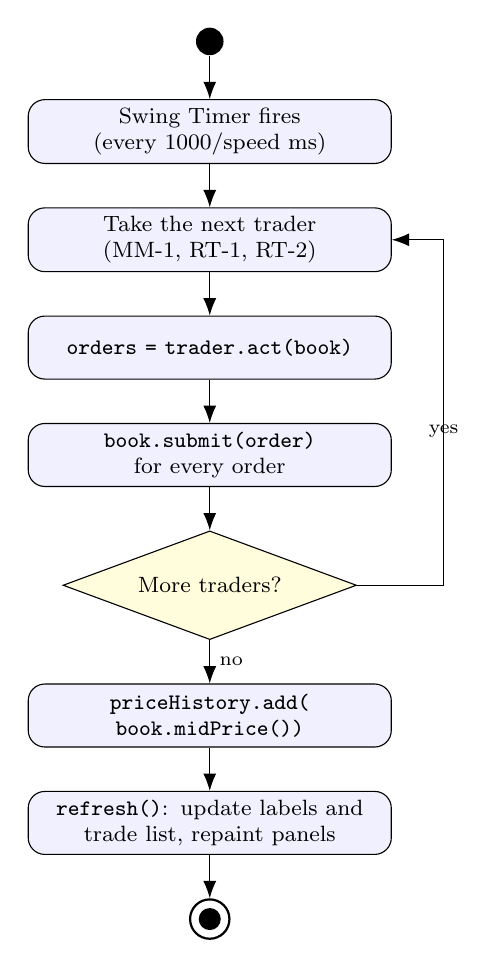
\begin{tikzpicture}[node distance=0.55cm,>={Latex[length=2.2mm]}]
\node[st] (s) {};
\node[act,below=of s] (a1) {Swing Timer fires\\(every $1000/\mathrm{speed}$ ms)};
\node[act,below=of a1] (a2) {Take the next trader\\(MM-1, RT-1, RT-2)};
\node[act,below=of a2] (a3) {\code{orders = trader.act(book)}};
\node[act,below=of a3] (a4) {\code{book.submit(order)}\\for every order};
\node[dec,below=of a4] (d1) {More traders?};
\node[act,below=of d1] (a5) {\code{priceHistory.add(}\\\code{book.midPrice())}};
\node[act,below=of a5] (a6) {\code{refresh()}: update labels and\\trade list, repaint panels};
\node[en,below=of a6] (e) {};
\draw[->] (s)--(a1); \draw[->] (a1)--(a2); \draw[->] (a2)--(a3); \draw[->] (a3)--(a4); \draw[->] (a4)--(d1);
\draw[->] (d1)--node[right,font=\scriptsize]{no}(a5);
\draw[->] (a5)--(a6); \draw[->] (a6)--(e);
\draw[->] (d1.east) -- ++(1.1,0) |- node[above,font=\scriptsize,pos=0.2]{yes} (a2.east);
\end{tikzpicture}}
\caption{Activity diagram of one simulation step.}
\label{fig:act-step}
\end{figure}

\begin{figure}[htbp]
\centering
\scalebox{0.88}{%
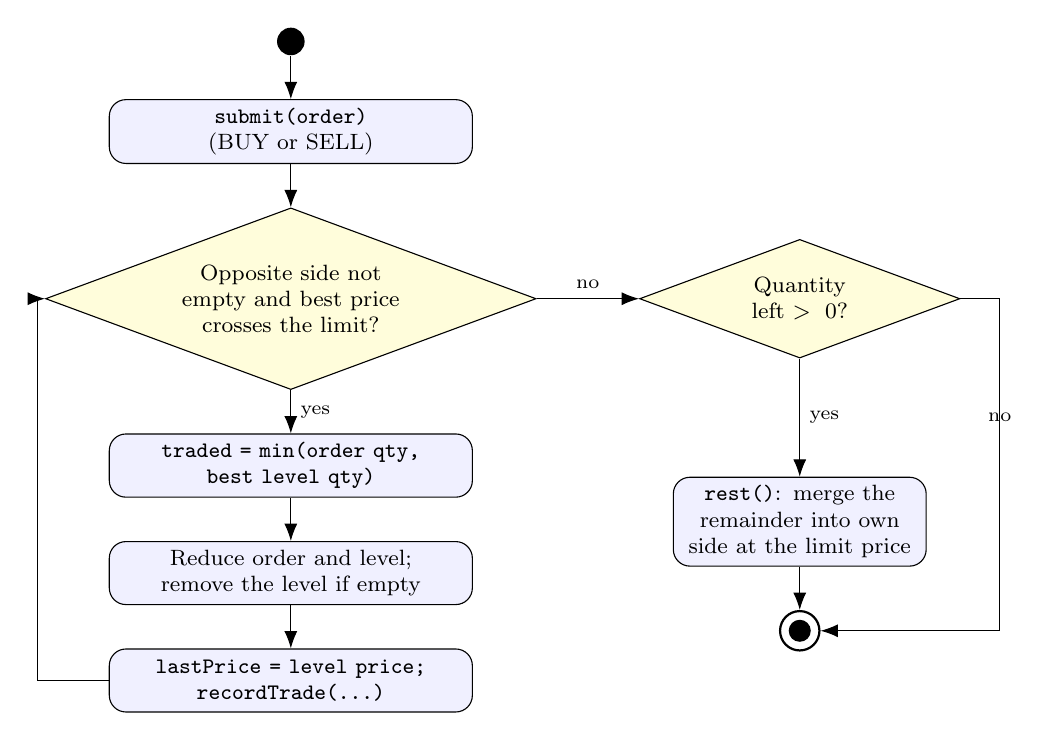
\begin{tikzpicture}[node distance=0.55cm,>={Latex[length=2.2mm]}]
\node[st] (s) {};
\node[act,below=of s] (b1) {\code{submit(order)}\\(BUY or SELL)};
\node[dec,below=of b1,text width=3.9cm] (d1) {Opposite side not\\empty and best price\\crosses the limit?};
\node[act,below=of d1] (b2) {\code{traded = min(order qty,}\\\code{best level qty)}};
\node[act,below=of b2] (b3) {Reduce order and level;\\remove the level if empty};
\node[act,below=of b3] (b4) {\code{lastPrice = level price;}\\\code{recordTrade(...)}};
\node[dec,right=1.3cm of d1,text width=2.6cm] (d2) {Quantity\\left $>0$?};
\node[act,below=1.5cm of d2,text width=3.0cm] (b5) {\code{rest()}: merge the\\remainder into own\\side at the limit price};
\node[en,below=of b5] (e) {};
\draw[->] (s)--(b1); \draw[->] (b1)--(d1);
\draw[->] (d1)--node[right,font=\scriptsize]{yes}(b2);
\draw[->] (b2)--(b3); \draw[->] (b3)--(b4);
\draw[->] (b4.west) -- ++(-0.9,0) |- (d1.west);
\draw[->] (d1.east)--node[above,font=\scriptsize]{no}(d2.west);
\draw[->] (d2.south)--node[right,font=\scriptsize]{yes}(b5.north);
\draw[->] (b5)--(e);
\draw[->] (d2.east) -- ++(0.5,0) |- node[above,font=\scriptsize,pos=0.2]{no} (e.east);
\end{tikzpicture}}
\caption{Activity diagram of order matching in the book (\code{OrderBook.submit()}).}
\label{fig:act-match}
\end{figure}

\begin{figure}[htbp]
\centering
\resizebox{0.86\linewidth}{!}{%
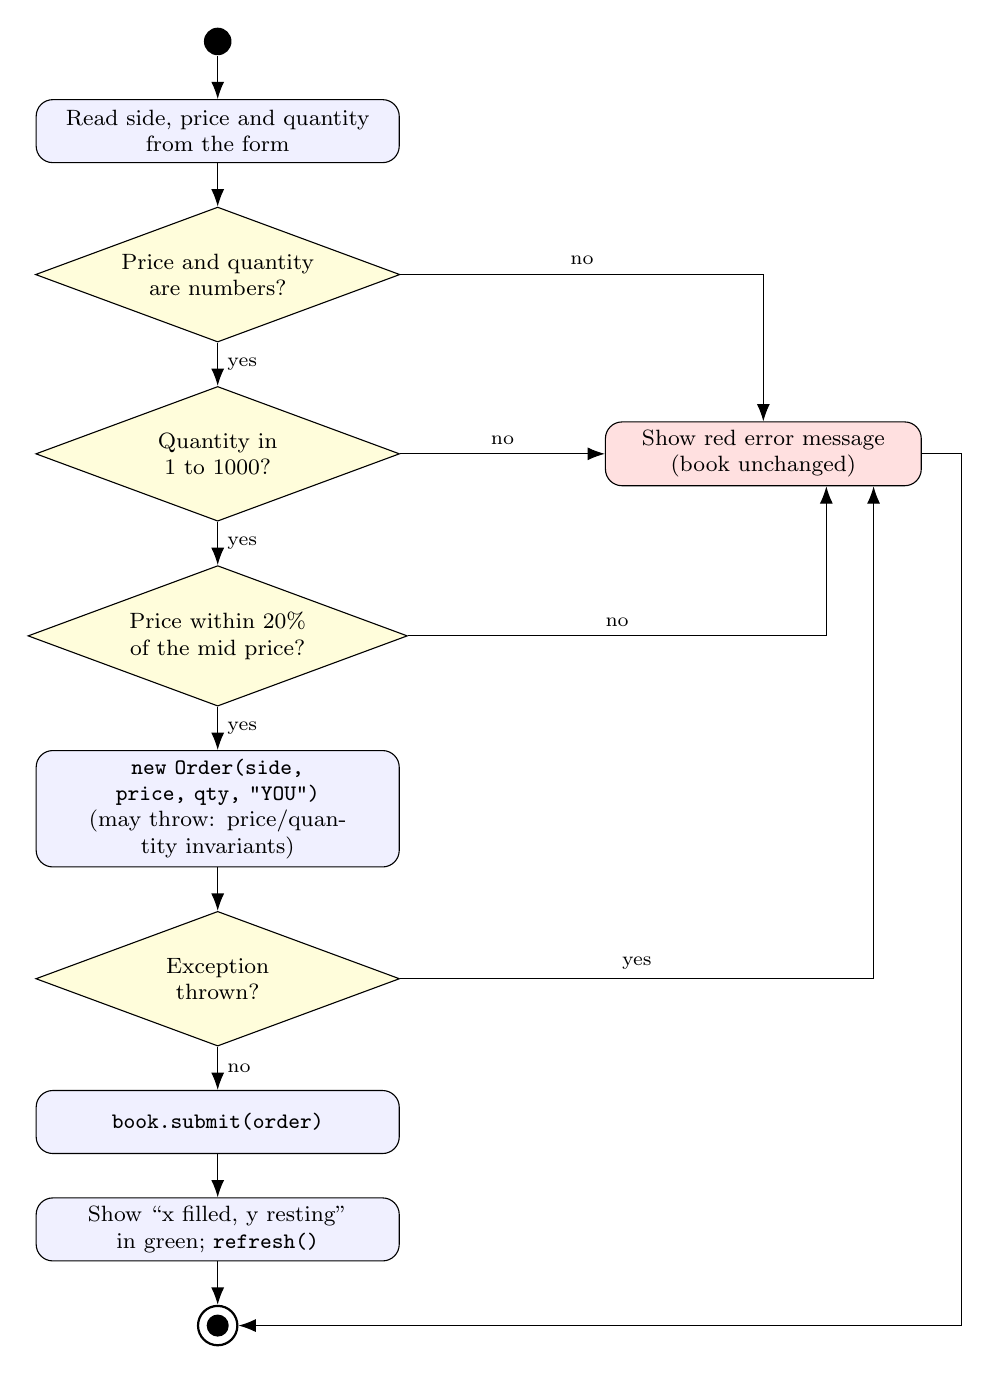
\begin{tikzpicture}[node distance=0.55cm,>={Latex[length=2.2mm]}]
\node[st] (s) {};
\node[act,below=of s] (c1) {Read side, price and quantity\\from the form};
\node[dec,below=of c1] (d1) {Price and quantity\\are numbers?};
\node[dec,below=of d1] (d2) {Quantity in\\1 to 1000?};
\node[dec,below=of d2] (d3) {Price within 20\%\\of the mid price?};
\node[act,below=of d3] (c2) {\code{new Order(side, price, qty, "YOU")}\\(may throw: price/quantity invariants)};
\node[dec,below=of c2] (d4) {Exception\\thrown?};
\node[act,below=of d4] (c3) {\code{book.submit(order)}};
\node[act,below=of c3] (c4) {Show ``x filled, y resting''\\in green; \code{refresh()}};
\node[en,below=of c4] (e) {};
\node[act,right=2.6cm of d2,fill=red!12,text width=3.8cm] (err) {Show red error message\\(book unchanged)};
\draw[->] (s)--(c1); \draw[->] (c1)--(d1);
\draw[->] (d1)--node[right,font=\scriptsize]{yes}(d2);
\draw[->] (d2)--node[right,font=\scriptsize]{yes}(d3);
\draw[->] (d3)--node[right,font=\scriptsize]{yes}(c2);
\draw[->] (c2)--(d4);
\draw[->] (d4)--node[right,font=\scriptsize]{no}(c3);
\draw[->] (c3)--(c4); \draw[->] (c4)--(e);
\draw[->] (d1.east) -| node[above,font=\scriptsize,pos=0.25]{no} (err.north);
\draw[->] (d2.east) -- node[above,font=\scriptsize]{no} (err.west);
\draw[->] (d3.east) -| node[above,font=\scriptsize,pos=0.25]{no} ([xshift=0.8cm]err.south);
\draw[->] (d4.east) -| node[above,font=\scriptsize,pos=0.25]{yes} ([xshift=1.4cm]err.south);
\draw[->] (err.east) -- ++(0.5,0) |- (e.east);
\end{tikzpicture}}
\caption{Activity diagram of the \emph{Place Order} action with validation.}
\label{fig:act-place}
\end{figure}

\section{Database Design / ER Diagram}

Not applicable. \projectTitle{} does not use a database: all state is held in memory while the window is open. The Java collections described in Table~\ref{tab:state} play the role of the data store.

\begin{table}[H]
\centering\small
\caption{In-memory data structures that hold the application state.}
\label{tab:state}
\begin{tabular}{@{}L{3.1cm} L{4.5cm} L{7.2cm}@{}}
\toprule
\textbf{Owner} & \textbf{Structure} & \textbf{Meaning}\\
\midrule
\code{OrderBook} & \code{TreeMap<Double,Integer> bids} & Price $\rightarrow$ total resting buy quantity, sorted from the highest price down.\\
\code{OrderBook} & \code{TreeMap<Double,Integer> asks} & Price $\rightarrow$ total resting sell quantity, sorted from the lowest price up.\\
\code{OrderBook} & \code{List<String> trades} & The 8 latest trades, newest first.\\
\code{OrderBook} & \code{double lastPrice} & Price of the most recent trade.\\
\code{MarketSimulator} & \code{List<Double> priceHistory} & Mid price after every step.\\
\code{MarketSimulator} & \code{List<Trader> traders} & The three simulated participants.\\
\bottomrule
\end{tabular}
\end{table}

\section{Module Description}

The system is divided into six modules (Table~\ref{tab:modules}). Each module has one clear responsibility and lives in a small number of classes.

\begin{table}[H]
\centering\small
\caption{Modules of \projectTitle{}.}
\label{tab:modules}
\begin{tabular}{@{}l L{2.9cm} L{3.3cm} L{5.4cm}@{}}
\toprule
\textbf{No.} & \textbf{Module} & \textbf{Classes} & \textbf{Responsibility}\\
\midrule
M1 & Order model & \code{Order}, \code{ImpactResult} & Describe an order and the result of an impact estimate; reject invalid prices and quantities.\\
M2 & Matching engine & \code{OrderBook} & Keep bids and asks, match marketable orders, rest the remainder, record trades, compute the mid price and estimate impact.\\
M3 & Trading agents & \code{Trader}, \code{MarketMaker}, \code{RandomTrader} & Decide which orders to submit each step.\\
M4 & Simulation controller & \code{MarketSimulator} & Own the book and the traders, run one step and record the price history.\\
M5 & Visualization & \code{PriceChartPanel}, \code{OrderBookPanel} & Paint the price chart and the depth ladder.\\
M6 & Window and controls & \code{MainFrame} & Build the window, run the timer, show statistics, handle the order form, pause and speed controls, and report errors.\\
\bottomrule
\end{tabular}
\end{table}

% =====================================================================
%  CHAPTER 3
% =====================================================================
\chapter{Implementation}

\section{Technologies and Tools Used}

\begin{table}[H]
\centering\small
\caption{Technologies and tools.}
\label{tab:tech}
\begin{tabular}{@{}L{3.6cm} L{4.2cm} L{6.9cm}@{}}
\toprule
\textbf{Technology / tool} & \textbf{Version} & \textbf{Purpose}\\
\midrule
Java (JDK) & OpenJDK 17 (Eclipse Temurin 17.0.9); only Java 8 language features are used & Programming language, compiler (\code{javac}) and runtime (\code{java}).\\
Java Swing / AWT & Part of the JDK & Window, panels, timer and 2D drawing (\code{JFrame}, \code{JPanel}, \code{Timer}, \code{Graphics2D}).\\
Java Collections Framework & Part of the JDK & \code{TreeMap}, \code{ArrayList}, \code{List}, \code{Map.Entry}, streams.\\
Git & -- & Version control of the source code.\\
XeLaTeX (TeX Live) & 2026 & Typesetting of this report.\\
macOS & 15 (Darwin 24) & Development and testing platform.\\
\bottomrule
\end{tabular}
\end{table}

No external libraries, frameworks or build tools are required. The project compiles with a single \code{javac} command.

\section{Project Structure / Package Structure}

All classes are in the default package and are grouped by relationship, one logical unit per file.

\begin{lstlisting}[style=plain]
project_java/
|-- Order.java             Order, ImpactResult
|-- Trader.java            Trader (abstract), MarketMaker, RandomTrader
|-- OrderBook.java         OrderBook
|-- MarketSimulator.java   MarketSimulator
|-- MainFrame.java         MainFrame, PriceChartPanel, OrderBookPanel
|-- readme.md              project description
|-- .gitignore             ignores *.class build artifacts
|-- report/                this report (LaTeX source, figures, PDF)
\end{lstlisting}

To compile and run the application:

\begin{lstlisting}[style=plain]
javac Order.java Trader.java OrderBook.java MarketSimulator.java MainFrame.java
java MainFrame
\end{lstlisting}

\section{Description of Classes and Interfaces}

Table~\ref{tab:classes} summarises every class. The project defines no Java interfaces of its own. The abstract class \code{Trader} is the extension point of the design: a new strategy only has to extend it and implement \code{act()}. The Swing listeners are implemented with lambda expressions, which Java treats as instances of the functional interfaces \code{ActionListener} and \code{ChangeListener}.

\begin{longtable}{@{}L{3.3cm} L{5.0cm} L{6.3cm}@{}}
\caption{Classes of the project.}\label{tab:classes}\\
\toprule
\textbf{Class (file)} & \textbf{Responsibility} & \textbf{Important members}\\
\midrule
\endfirsthead
\toprule
\textbf{Class (file)} & \textbf{Responsibility} & \textbf{Important members}\\
\midrule
\endhead
\bottomrule
\endfoot
\code{Order}\newline{\footnotesize Order.java} & One order. Everything is final except the remaining quantity. The constructor validates the price and the quantity. & \code{enum Side \{BUY, SELL\}}, \code{getSide()}, \code{getPrice()}, \code{getQuantity()}, \code{setQuantity()}, \code{getTraderId()}, \code{toString()}\\
\code{ImpactResult}\newline{\footnotesize Order.java} & Result of an impact estimate: filled quantity, average fill price and price impact. & \code{getFilledQuantity()}, \code{getAvgFillPrice()}, \code{getPriceImpact()}, \code{toString()}\\
\code{OrderBook}\newline{\footnotesize OrderBook.java} & The matching engine and the state of the book. & \code{submit()}, \code{matchBuy()}, \code{matchSell()}, \code{rest()}, \code{reduce()}, \code{recordTrade()}, \code{bestBid()}, \code{bestAsk()}, \code{midPrice()}, \code{estimateImpact()}, \code{getBids()}, \code{getAsks()}, \code{getTrades()}\\
\code{Trader}\newline{\footnotesize Trader.java} & Abstract base class of all agents; holds id, cash and inventory. & \code{abstract List<Order> act(OrderBook)}\\
\code{MarketMaker}\newline{\footnotesize Trader.java} & Quotes both sides around the mid price. & \code{spread} (2.0), \code{quoteSize} (50), \code{act()}\\
\code{RandomTrader}\newline{\footnotesize Trader.java} & Submits one random order per step. & \code{rng}, \code{maxSize} (10), \code{act()}\\
\code{MarketSimulator}\newline{\footnotesize MarketSimulator.java} & Owns the book, the traders and the price history; runs one step. & \code{step()}, \code{getBook()}, \code{getPriceHistory()}, \code{getTraders()}\\
\code{MainFrame}\newline{\footnotesize MainFrame.java} & The window: layout, timer, statistics, order form, pause and speed controls, error messages. & \code{placeOrder()}, \code{estimateImpact()}, \code{readPrice()}, \code{readQuantity()}, \code{showMessage()}, \code{togglePause()}, \code{changeSpeed()}, \code{refresh()}, \code{main()}\\
\code{PriceChartPanel}\newline{\footnotesize MainFrame.java} & Paints the mid-price line chart. & \code{paintComponent()}\\
\code{OrderBookPanel}\newline{\footnotesize MainFrame.java} & Paints the depth ladder. & \code{paintComponent()}, \code{topLevels()}, \code{drawLevels()}\\
\end{longtable}

\section{Implementation of Major Modules}

\subsection{Matching engine (OrderBook)}

The book stores each side as a \code{TreeMap<Double,Integer>} that maps a price to the total quantity resting at that price. The bid map is created with \code{Collections.reverseOrder()}, so its first entry is the highest bid; the ask map uses the natural order, so its first entry is the lowest ask. \code{TreeMap} is a red--black tree, so inserting, removing and reading the first entry all take $O(\log n)$ time \cite{treemapapi,clrs}.

\code{submit()} looks at the side of the order. For a BUY it calls \code{matchBuy()}: while the order still has quantity, the ask side is not empty and the order price is at least the best ask, it trades \code{min(order quantity, best level quantity)}, reduces both the order and the level (removing the level when it reaches zero), updates \code{lastPrice} and records the trade. A SELL works the same way against the bids. Every trade executes at the \emph{resting} order's price, so an aggressive order gets price improvement when it crosses several levels. Whatever quantity is left after matching is added to the order's own side with \code{TreeMap.merge()}. An order that sweeps $k$ levels costs $O(k\log n)$.

\code{midPrice()} returns the average of the best bid and best ask; if only one side exists it returns that side's best price, and if the book is empty it returns the last trade price. \code{estimateImpact()} walks the opposite side from the best price, adding up quantity and notional value until the requested size is covered, and returns the filled quantity, the average fill price and the \emph{impact}, defined as the price of the deepest level touched minus the current mid price. It never modifies the book.

\subsection{Trading agents (Trader, MarketMaker, RandomTrader)}

\code{Trader} declares the single abstract method \code{List<Order> act(OrderBook book)}. The \textbf{market maker} reads the mid price and returns two orders: a BUY of 50 units at $\text{mid}-1.0$ and a SELL of 50 units at $\text{mid}+1.0$ (spread 2.0). It never crosses the book by itself and keeps adding liquidity. A \textbf{random trader} returns one order per step: a random side, a quantity from 1 to 10 and a price of $\text{mid}\pm\text{offset}$ with offset 0, 1 or 2, where a buyer pays \emph{above} the mid and a seller asks \emph{below} it. Such orders are often marketable and therefore trade against the market maker's quotes, which is what moves the price. Both random traders share one \code{Random} instance created with seed 42.

\subsection{Simulation loop (MarketSimulator)}

The simulator is created with an initial price of 100.0, builds the book, registers \code{MM-1}, \code{RT-1} and \code{RT-2} in that order and stores the initial price as the first history entry. \code{step()} lets each trader act in order and submits its orders immediately, so later traders see the effect of earlier ones, and finally appends the new mid price to the history. Because the random generator is seeded and the traders act in a fixed order, the sequence of steps is identical in every run, which makes demonstrations repeatable.

\subsection{Price chart (PriceChartPanel)}

The panel draws the last 200 mid prices. It finds the minimum and maximum of that window and pads the range by 10\% of its width (at least 0.05) so the line does not touch the edges. With the plot area at $x_\text{left}=56$ and $y_\text{top}=32$ pixels, width $w$ and height $h$, point $i$ of $n$ is placed at
\[
x_i = x_\text{left} + \frac{i}{n-1}\,w,\qquad
y_i = y_\text{top} + \frac{p_\text{max}-p_i}{p_\text{max}-p_\text{min}}\,h .
\]
Five horizontal grid lines carry price labels, the line is drawn with a 2-pixel antialiased stroke and the latest point is marked with a dot.

\subsection{Depth ladder (OrderBookPanel)}

The panel collects the first 10 entries of each side. The asks are reversed so that the best ask is at the bottom of the red block, directly above the best bid, with a divider line marking the spread. A bar's length is $\text{quantity}/\text{maxQuantity}\times(\text{panel width}-110)$ pixels, where \code{maxQuantity} is the largest quantity among the displayed levels, and the quantity is written at the end of the bar. Asks are red and bids are green. The block of asks is shifted down when fewer than 10 levels exist, so the divider stays at the same height.

\subsection{Window and controls (MainFrame)}

\code{MainFrame} uses a \code{BorderLayout}: the statistics row at the top, the chart in the centre, the depth ladder with the trade list on the right and the control panel at the bottom. Its timer is created with a 200~ms delay. \code{refresh()} fills the labels from the book, writes the trades into a read-only text area and repaints both panels; it is called after every timer step and after every user order. The \emph{Pause} button stops or restarts the timer, and the speed slider calls \code{timer.setDelay(1000 / steps)}. The order form's \emph{Place Order} and \emph{Estimate Impact} buttons, and the Enter key in the price and quantity fields, call \code{placeOrder()} and \code{estimateImpact()}. Results are shown in a message line under the controls: green for success and red for errors.

\section{Exception Handling}

User input is the only source of errors in the application, so the form handlers wrap their work in \code{try}/\code{catch} blocks and turn every failure into a message in the window (Table~\ref{tab:exceptions}). Validation happens at two levels. The \textbf{engine} protects its own invariants: the \code{Order} constructor throws \code{IllegalArgumentException} for a price that is not a positive finite number or a quantity of zero or less, so an invalid order can never reach the book, even when the engine is used without the GUI. The \textbf{form} applies the rules of the demo: the quantity must be between 1 and 1000, and the price must be within 20\% of the current mid price. This ``fat-finger'' check stops a typing mistake such as \code{10000} from creating a huge resting order that the market maker would then follow. The standard \code{IllegalArgumentException} is used for rule violations, as recommended in \cite{exceptionstutorial,effectivejava}.

\begin{table}[H]
\centering\small
\caption{Validation rules and the exceptions that implement them.}
\label{tab:exceptions}
\begin{tabular}{@{}L{3.5cm} L{2.8cm} L{3.5cm} L{4.6cm}@{}}
\toprule
\textbf{Invalid input} & \textbf{Detected in} & \textbf{Exception} & \textbf{Message shown}\\
\midrule
Price is not a number & \code{readPrice()} & \code{NumberFormat\-Exception} & Price and quantity must be numbers\\
Quantity is not an integer & \code{readQuantity()} & \code{NumberFormat\-Exception} & Price and quantity must be numbers (Place Order); Quantity must be a number (Estimate Impact)\\
Quantity outside 1--1000 & \code{readQuantity()} & \code{IllegalArgument\-Exception} & Quantity must be between 1 and 1000\\
Price more than 20\% from the mid & \code{readPrice()} & \code{IllegalArgument\-Exception} & Price must be within 20\% of the mid price (\emph{mid})\\
Price is NaN, infinite or $\le 0$ & \code{Order} constructor & \code{IllegalArgument\-Exception} & Price must be a positive number\\
Quantity $\le 0$ & \code{Order} constructor & \code{IllegalArgument\-Exception} & Quantity must be greater than 0\\
\bottomrule
\end{tabular}
\end{table}

\code{NumberFormatException} is a subclass of \code{IllegalArgumentException}, so the \code{catch} block for \code{NumberFormatException} must come first; otherwise the more general block would swallow it and the user would see the wrong message. Two details are worth noting. The text \code{Infinity} is rejected by the 20\% check, whereas \code{NaN} passes that comparison (every comparison with \code{NaN} is false) and is rejected by the \code{Order} constructor, which is why the constructor performs its own check. An inline message line is used instead of a pop-up dialog so that the simulation stays visible and the user can correct the value at once. No checked exceptions are involved and no resources need to be closed.

\section{Collection Framework Usage}

The Java Collections Framework \cite{collectionstutorial} is the backbone of the project (Table~\ref{tab:collections}). The most important choice is the \code{TreeMap}: because the map keeps its keys sorted, the best bid and best ask are always the first entry, and a single comparator (\code{Collections.reverseOrder()}) is enough to turn the same data structure into a descending bid book.

\begin{table}[H]
\centering\small
\caption{Use of the Collections Framework.}
\label{tab:collections}
\begin{tabular}{@{}L{4.6cm} L{3.2cm} L{6.6cm}@{}}
\toprule
\textbf{Collection / API} & \textbf{Where} & \textbf{Why}\\
\midrule
\code{TreeMap<Double,\allowbreak Integer>} with \code{Collections.\allowbreak reverseOrder()} & \code{OrderBook.\allowbreak bids} & Sorted from the highest price; \code{firstEntry()} is the best bid in $O(\log n)$.\\
\code{TreeMap<Double,\allowbreak Integer>} & \code{OrderBook.\allowbreak asks} & Sorted from the lowest price; \code{firstEntry()} is the best ask.\\
\code{TreeMap.merge()}, \code{getOrDefault()}, \code{put()}, \code{remove()} & \code{rest()}, \code{reduce()} & Add quantity to a level, reduce it, or delete an empty level.\\
\code{ArrayList<Double>} & \code{MarketSimulator.\allowbreak priceHistory} & Append one mid price per step; \code{subList()} gives the last 200 points to the chart.\\
\code{ArrayList<Trader>} & \code{MarketSimulator.\allowbreak traders} & A polymorphic list that keeps the traders in a fixed order.\\
\code{ArrayList<Order>} & return value of \code{act()} & The orders a trader wants to submit in one step.\\
\code{ArrayList<String>} & \code{OrderBook.trades} & The latest 8 trades; \code{add(0, \ldots)} puts the newest first.\\
\code{Map.Entry}, \code{ArrayList<Map.\allowbreak Entry<\ldots>>}, \code{Collections.\allowbreak reverse()} & \code{OrderBookPanel} & Take the top 10 levels of a side and flip the asks for display.\\
Streams (\code{mapToDouble().\allowbreak min()/max()}) & \code{PriceChartPanel} & Find the price range of the plotted window.\\
\code{Order.Side.values()} & \code{MainFrame.\allowbreak sideBox} & Fill the BUY/SELL combo box from the enum.\\
\code{String.join()} & \code{MainFrame.\allowbreak refresh()} & Turn the trade list into the text of the trade panel.\\
\bottomrule
\end{tabular}
\end{table}

\section{Database Connectivity}

Not applicable. The application does not connect to a database. If persistence were added later, the trade list and the price history could be stored through JDBC (for example in SQLite); the current design already isolates the state in \code{OrderBook} and \code{MarketSimulator}, which would make that change local.

\section{Important Code Snippets}

The listings below are the real source code of the project.

\subsection*{Order validation}
The constructor refuses orders that could corrupt the book.
\keeplisting[firstline=14,lastline=25,firstnumber=14,caption={\code{Order} constructor (Order.java).},label={lst:order}]{../Order.java}

\subsection*{Order matching and resting}
\code{submit()} dispatches on the side; \code{matchBuy()} trades against the best asks while the price crosses; leftover quantity rests in the book.
\keeplisting[firstline=23,lastline=47,firstnumber=23,caption={\code{OrderBook.submit()} and \code{matchBuy()} (OrderBook.java).},label={lst:match}]{../OrderBook.java}

\keeplisting[firstline=61,lastline=79,firstnumber=61,caption={Resting, reducing a level and recording a trade (OrderBook.java).},label={lst:rest}]{../OrderBook.java}

\subsection*{Market impact estimate}
The estimate walks the book without changing it.
\keeplisting[firstline=95,lastline=112,firstnumber=95,caption={\code{OrderBook.estimateImpact()} (OrderBook.java).},label={lst:impact}]{../OrderBook.java}

\subsection*{Trading agents}
\keeplisting[firstline=43,lastline=50,firstnumber=43,caption={\code{MarketMaker.act()} (Trader.java).},label={lst:mm}]{../Trader.java}

\keeplisting[firstline=67,lastline=77,firstnumber=67,caption={\code{RandomTrader.act()} (Trader.java).},label={lst:rt}]{../Trader.java}

\subsection*{Simulation step}
\keeplisting[firstline=24,lastline=31,firstnumber=24,caption={\code{MarketSimulator.step()} (MarketSimulator.java).},label={lst:step}]{../MarketSimulator.java}

\subsection*{User input handling}
\code{placeOrder()} shows the two-level validation: the readers throw for rule violations and the \code{catch} blocks turn every failure into a message.
\keeplisting[firstline=171,lastline=187,firstnumber=171,caption={\code{MainFrame.placeOrder()} (MainFrame.java).},label={lst:place}]{../MainFrame.java}

\keeplisting[firstline=202,lastline=218,firstnumber=202,caption={Input readers with range checks (MainFrame.java).},label={lst:read}]{../MainFrame.java}

% =====================================================================
%  CHAPTER 4
% =====================================================================
\chapter{Results and Screenshots}

All screenshots in this chapter were taken from the running application. They come from one repeatable session: the simulation was run for 150 steps with the fixed seed and the actions below were then performed one after another, so the numbers quoted in the text can be read directly from the figures.

\section{Main Application Screen}

Figure~\ref{fig:main} shows the window after 150 simulation steps. The regions marked A to G are described in Table~\ref{tab:regions}.

\begin{figure}[htbp]
\centering
\begin{tikzpicture}
\node[anchor=south west,inner sep=0] (img) at (0,0) {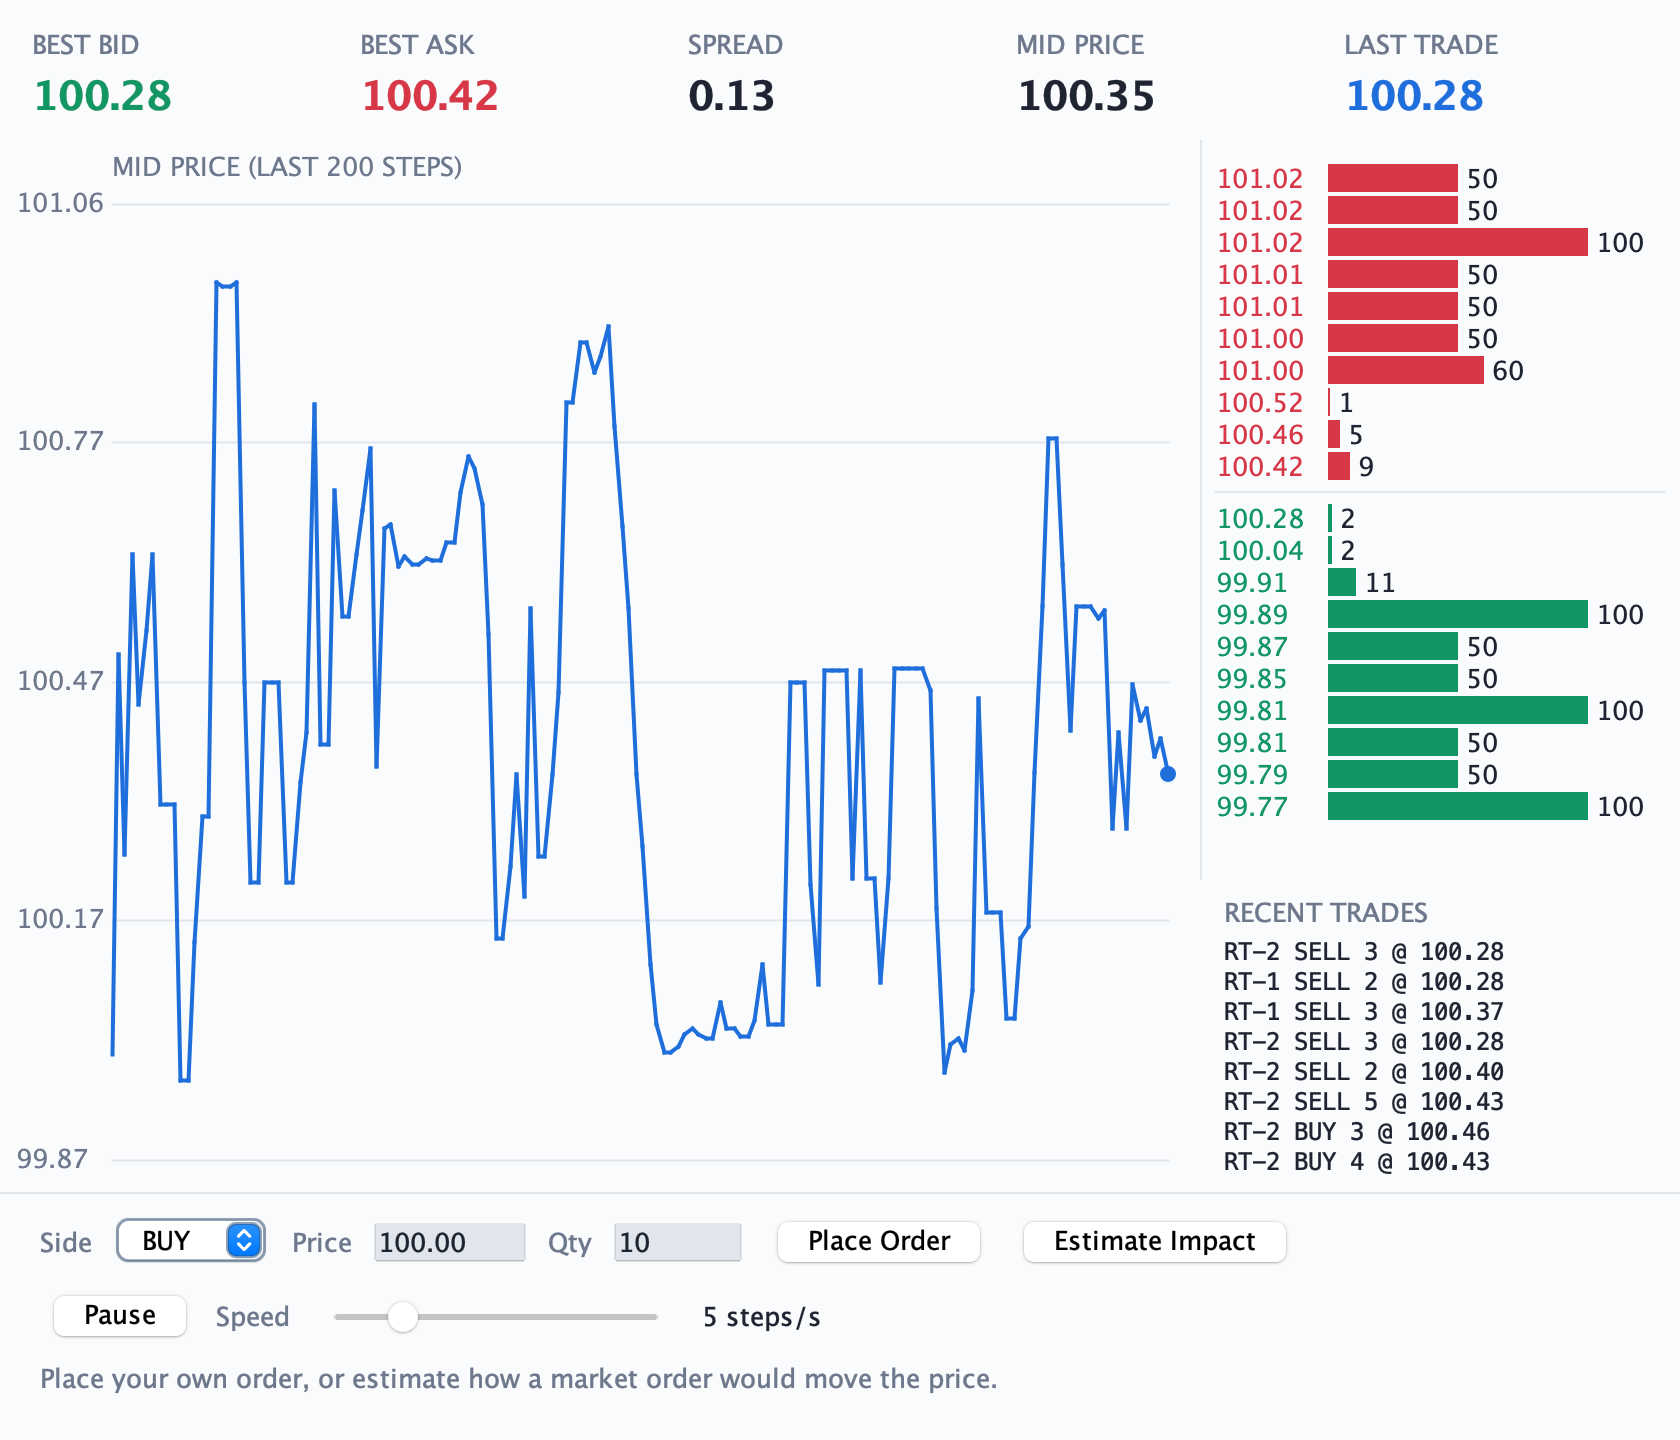
\includegraphics[width=13.6cm]{figures/fig_main.png}};
\newcommand{\badge}[3]{\node[badge] at ($(img.south west)+({#2*0.008095},{(1440-#3)*0.008095})$) {#1};}
\badge{A}{1625}{75}
\badge{B}{660}{168}
\badge{C}{1575}{518}
\badge{D}{1625}{912}
\badge{E}{1400}{1243}
\badge{F}{1000}{1317}
\badge{G}{1250}{1380}
\draw[black!30] (img.south west) rectangle (img.north east);
\end{tikzpicture}
\caption{Main screen of \projectTitle{} (light theme) after 150 steps.}
\label{fig:main}
\end{figure}

\begin{table}[H]
\centering\small
\caption{Regions of the main screen.}
\label{tab:regions}
\begin{tabular}{@{}c L{3.6cm} L{9.6cm}@{}}
\toprule
\textbf{Mark} & \textbf{Region} & \textbf{Content}\\
\midrule
A & Statistics row & Best bid (green), best ask (red), spread, mid price and last trade price. Here: 100.28, 100.42, 0.13, 100.35 and 100.28.\\
B & Price chart & Mid price of the last 200 steps with price labels and grid lines; the dot marks the latest value.\\
C & Depth ladder & Top 10 ask levels (red) above top 10 bid levels (green); bar length shows the quantity.\\
D & Recent trades & The 8 latest trades as \emph{trader, side, quantity @ price}.\\
E & Order form & Side, price and quantity fields with the \emph{Place Order} and \emph{Estimate Impact} buttons.\\
F & Simulation controls & \emph{Pause/Resume} button and the speed slider (1--20 steps per second).\\
G & Message line & Green result of the last action, or a red error message.\\
\bottomrule
\end{tabular}
\end{table}

\section{Functional Screenshots}

\subsection{Live statistics, chart and depth}

Figure~\ref{fig:parts} shows the chart panel and the depth ladder with the trade list at full size. The market maker's quotes of 50 units each are visible as the regular bars; the larger bars (100 and 150) are levels where several quotes accumulated at nearly the same price.

\begin{figure}[htbp]
\centering
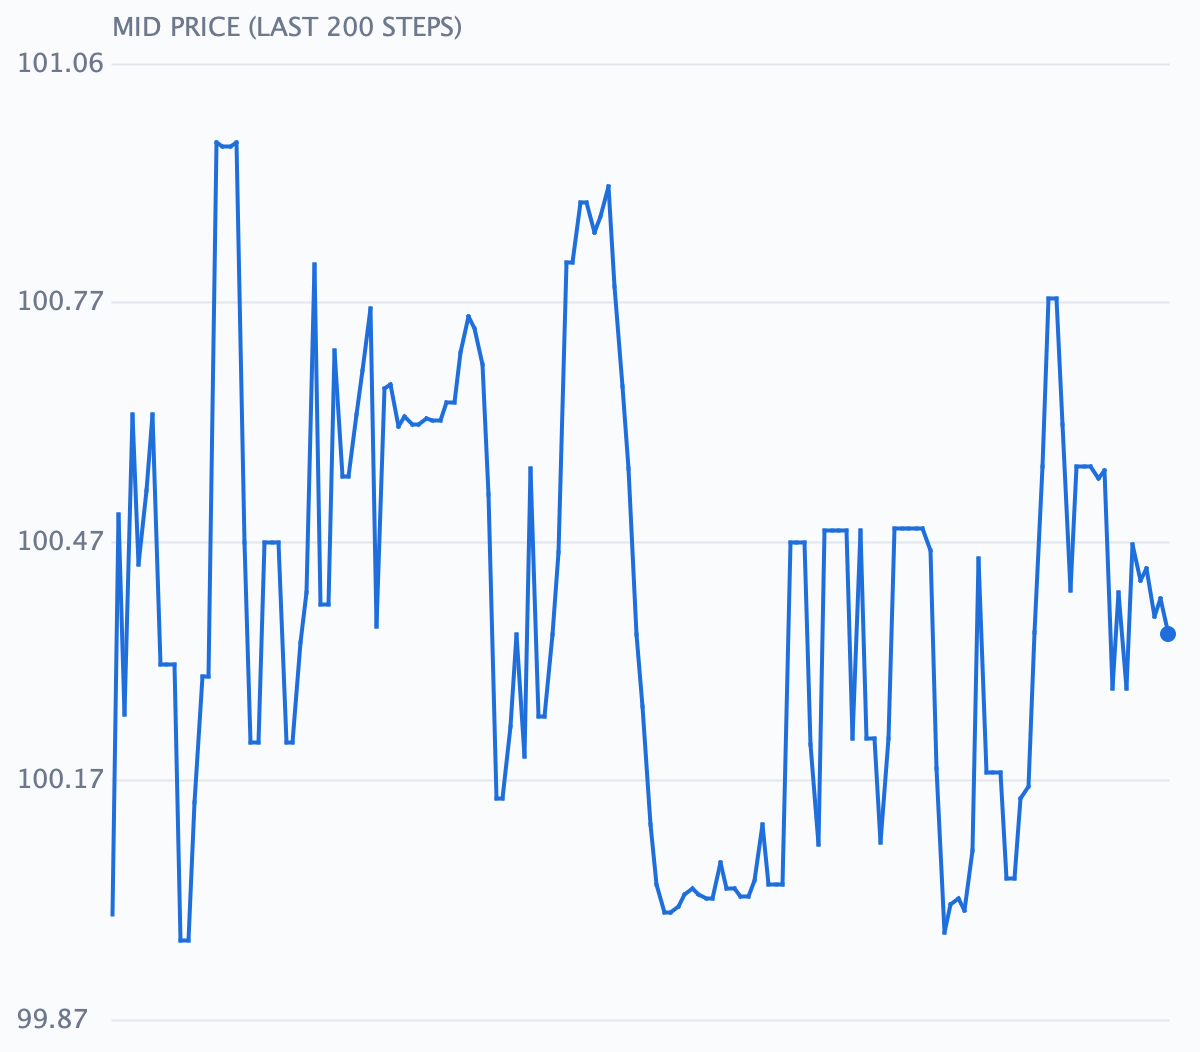
\includegraphics[height=7.6cm]{figures/fig_chart.png}\hfill
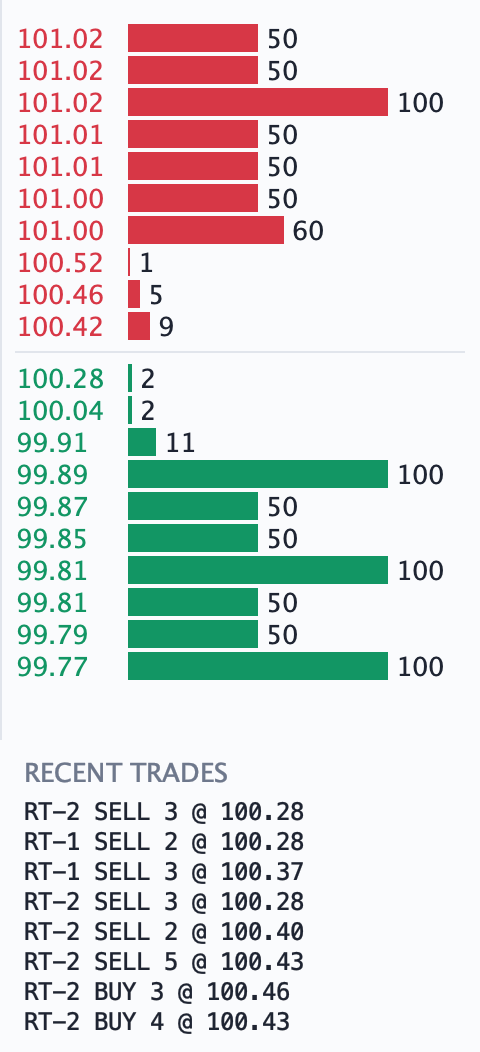
\includegraphics[height=7.6cm]{figures/fig_book.png}
\caption{Left: price chart panel. Right: depth ladder and recent trades.}
\label{fig:parts}
\end{figure}

\subsection{Placing a marketable order}

Before this action the best ask was 100.42 and the mid price 100.35 (Figure~\ref{fig:main}). A BUY of 120 units with a limit price of 101.42 is marketable, so it is matched immediately (Figure~\ref{fig:filled}). The message reads \emph{BUY 120 @ 101.42: 120 filled, 0 resting}. The trade list shows that the order walked up the ask side in five trades: 9 @ 100.42, 5 @ 100.46, 1 @ 100.52, 60 @ 101.00 and 45 @ 101.00, which add up to 120. Every trade is at the price of the level that was consumed, not at the buyer's limit of 101.42. The best ask moved from 100.42 to 101.00, the spread widened from 0.13 to 0.72 and the mid price rose from 100.35 to 100.64.

\begin{figure}[htbp]
\centering
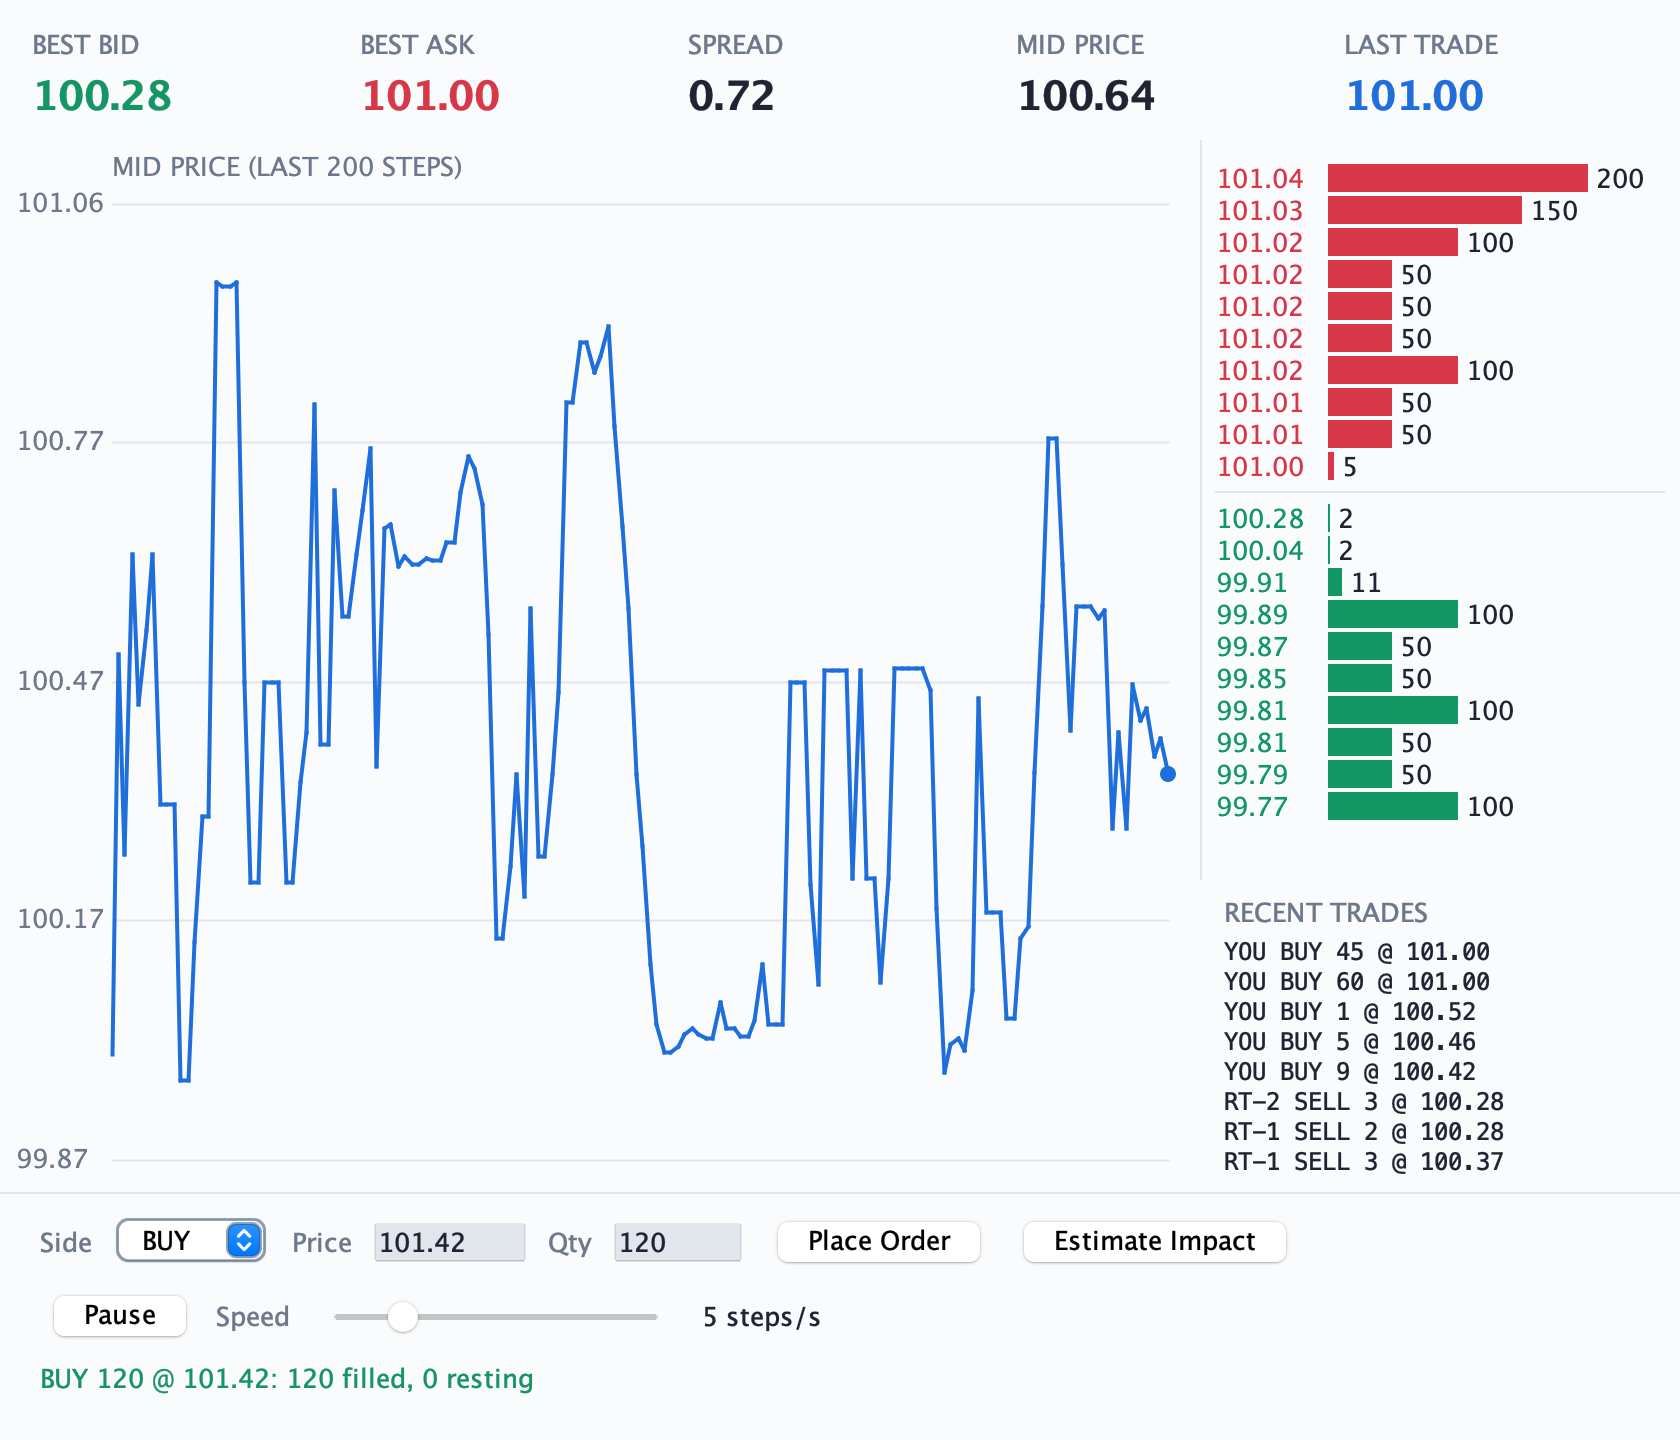
\includegraphics[width=0.82\linewidth]{figures/fig_order_filled.png}
\caption{After placing BUY 120 @ 101.42: the order is fully filled and the ask side has moved up.}
\label{fig:filled}
\end{figure}

\subsection{Placing a resting order}

A BUY of 40 units at 100.23 is below the best ask (101.00), so nothing trades (Figure~\ref{fig:resting}). The message reads \emph{BUY 40 @ 100.23: 0 filled, 40 resting}, and a new bid level of 40 units appears at 100.23, directly below the best bid of 100.28. The statistics row is unchanged because the order did not improve the best bid.

\begin{figure}[htbp]
\centering
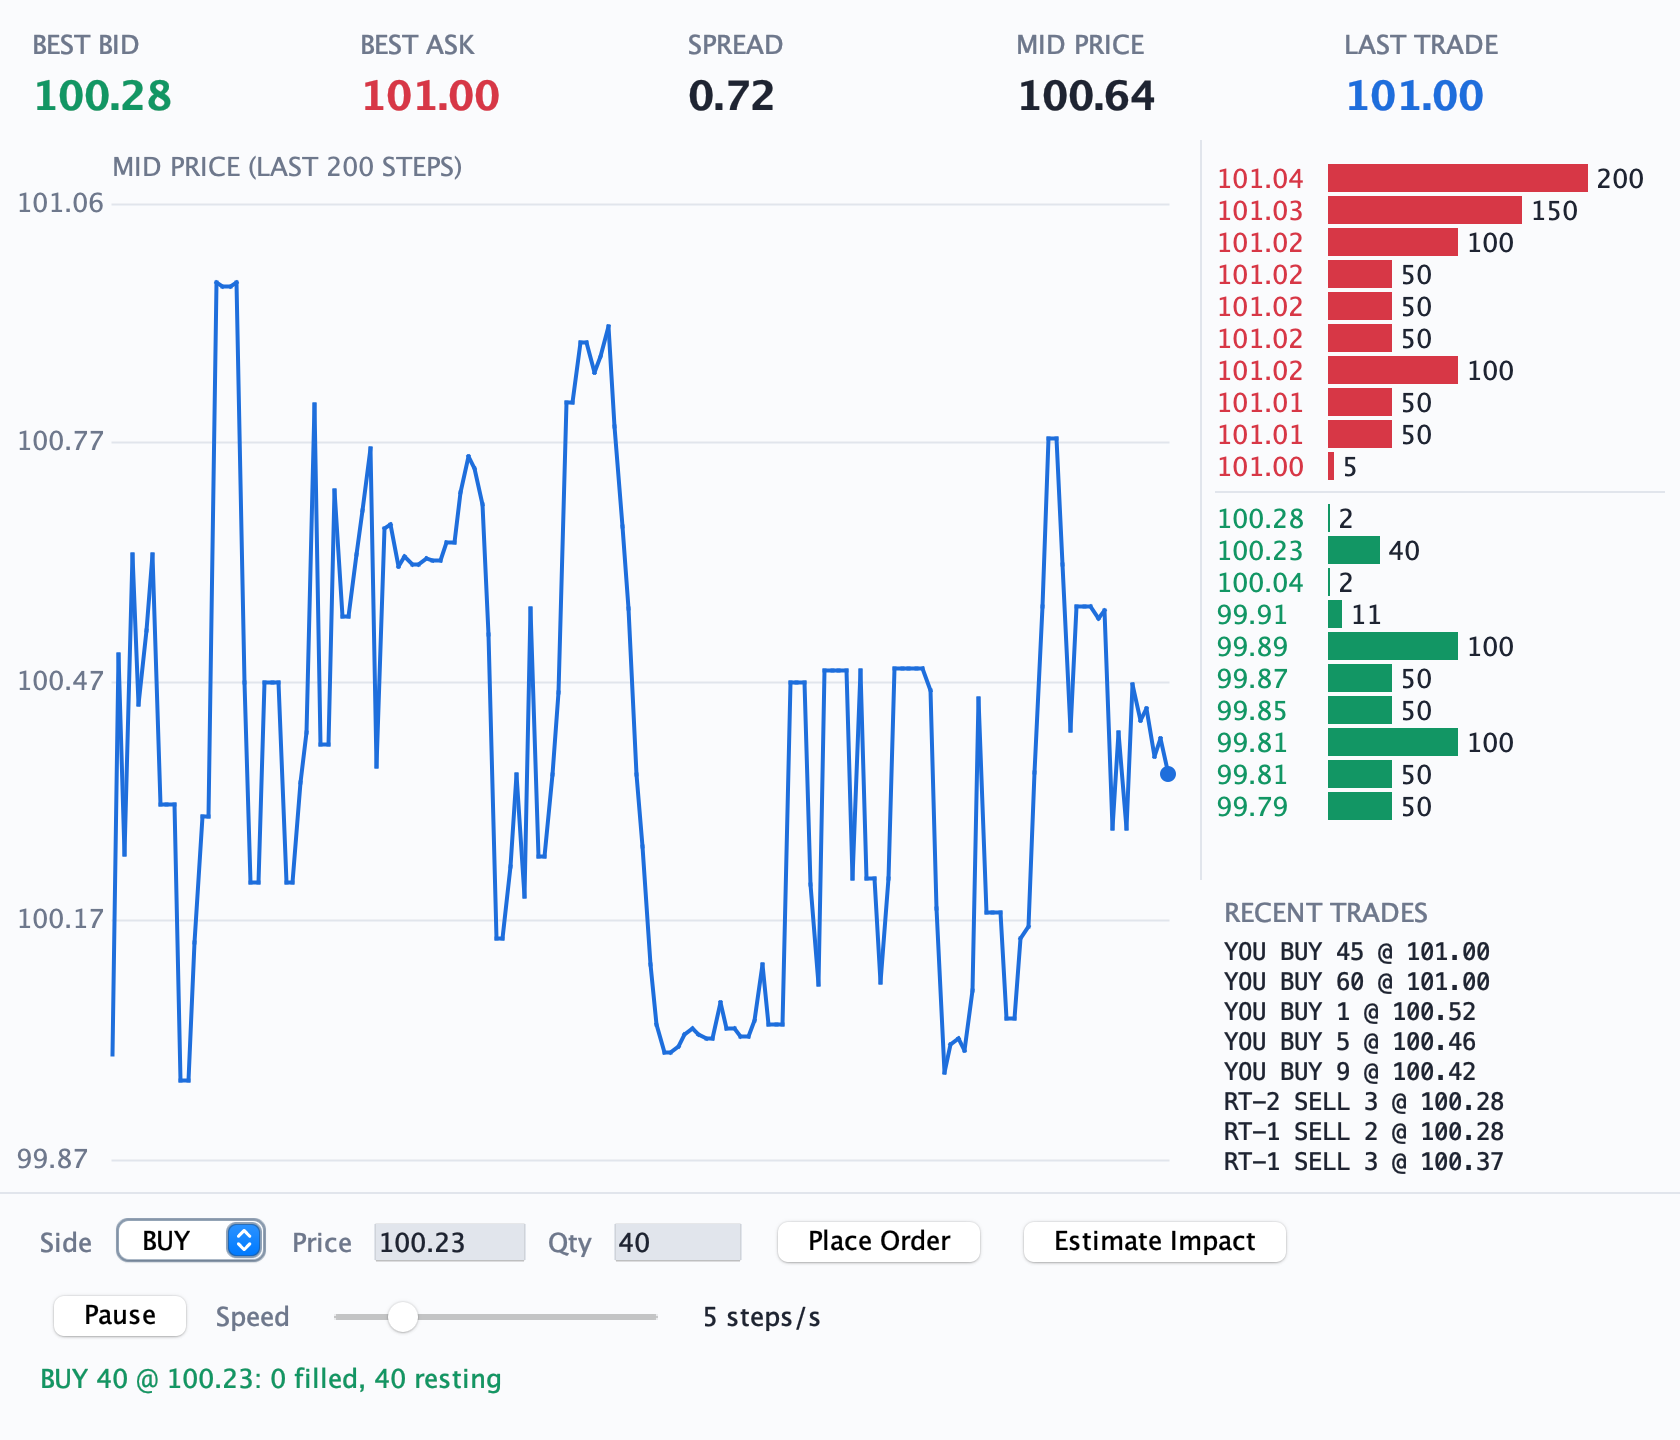
\includegraphics[width=0.82\linewidth]{figures/fig_order_resting.png}
\caption{After placing BUY 40 @ 100.23: the order rests as a new bid level.}
\label{fig:resting}
\end{figure}

\subsection{Estimating market impact}

With the side set to BUY and a quantity of 300, \emph{Estimate Impact} reports \emph{BUY 300 at market: filled=300 avg=101.02 impact=0.38} (Figure~\ref{fig:estimate}). In words: 300 units could be bought for an average price of 101.02, and the deepest level needed is 0.38 above the current mid price of 100.64. The book and the trade list are not changed by an estimate.

\begin{figure}[htbp]
\centering
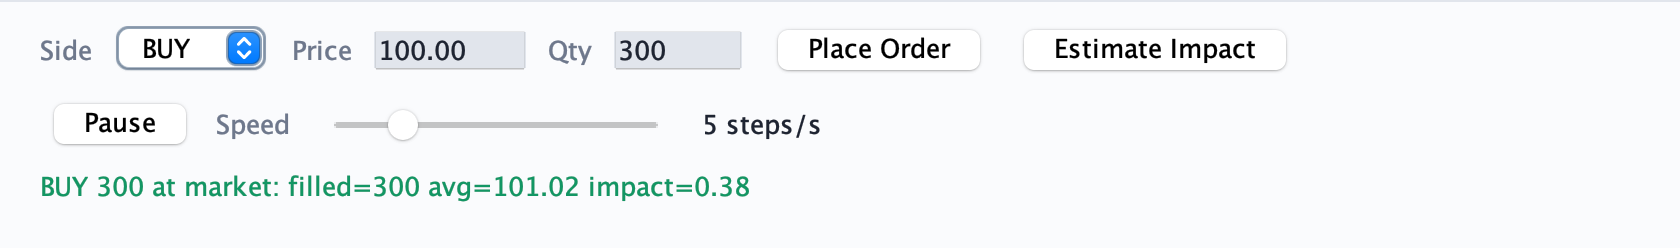
\includegraphics[width=\linewidth]{figures/fig_estimate.png}
\caption{Control panel after \emph{Estimate Impact} for BUY 300.}
\label{fig:estimate}
\end{figure}

\subsection{Effect of a large order}

A SELL of 1000 units with a limit of 85.55 (about 15\% below the mid price, inside the 20\% limit) sweeps the bid side (Figure~\ref{fig:sweep}). The message reads \emph{SELL 1000 @ 85.55: 1000 filled, 0 resting}; the trade list shows the last fills at 99.66--99.75. The best bid dropped from 100.28 to 99.66, the spread widened from 0.72 to 1.34 and the mid price fell from 100.64 to 100.33. The order also consumed the 40 units that the user had rested at 100.23, because the engine has no self-trade prevention. After 40 more steps (Figure~\ref{fig:sweep-after}) the market maker has quoted around the new level: the spread has narrowed to 0.55 and the mid price is 99.94.

\begin{figure}[htbp]
\centering
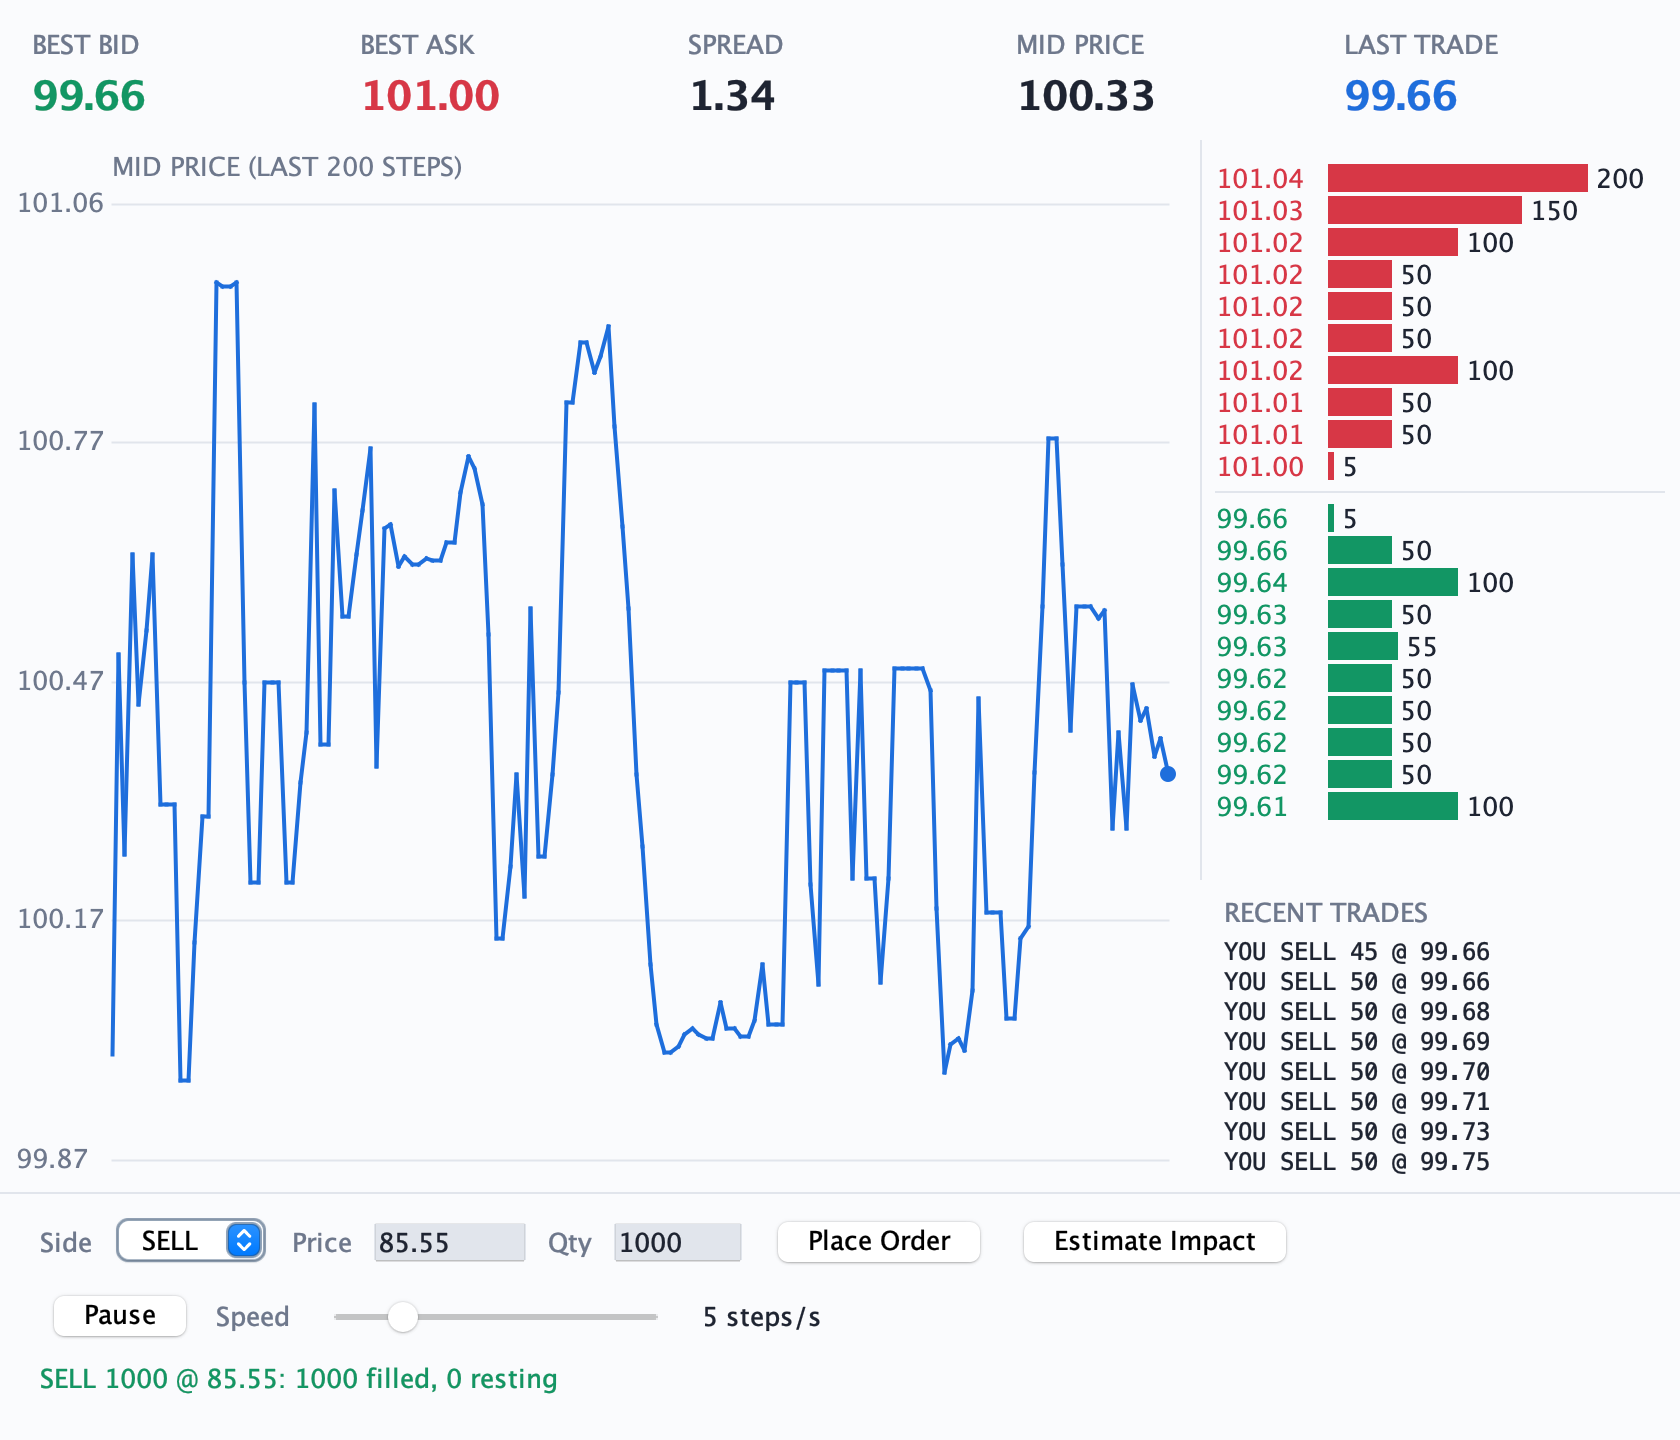
\includegraphics[width=0.78\linewidth]{figures/fig_sweep.png}
\caption{Immediately after SELL 1000 @ 85.55: the bid side has been consumed.}
\label{fig:sweep}
\end{figure}

\begin{figure}[htbp]
\centering
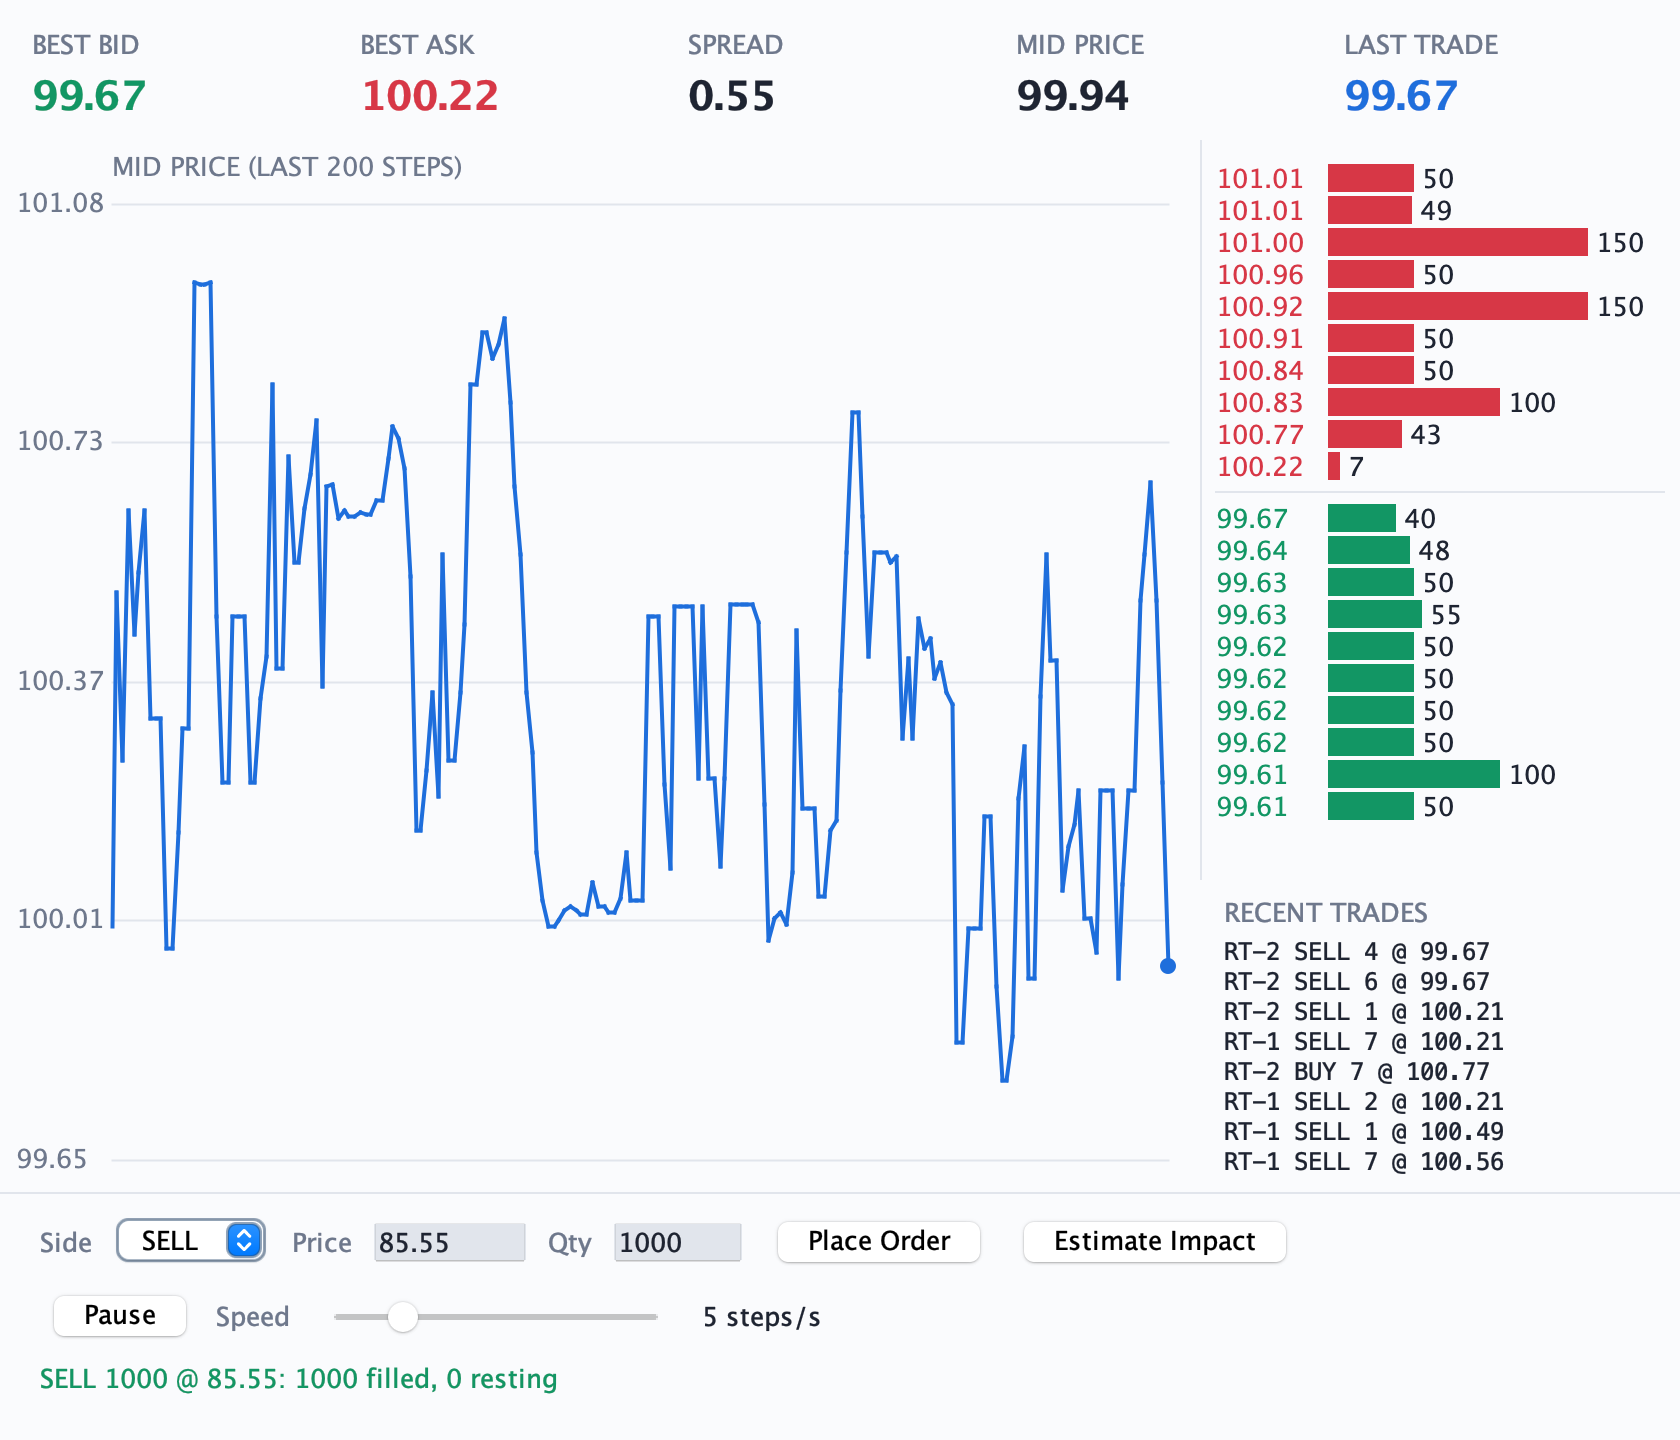
\includegraphics[width=0.78\linewidth]{figures/fig_sweep_after.png}
\caption{Forty simulation steps later: the market maker has rebuilt the quotes and the spread has narrowed.}
\label{fig:sweep-after}
\end{figure}

\subsection{Pause, resume and speed}

The \emph{Pause} button stops the timer and turns into \emph{Resume}; the speed slider changes the number of steps per second, shown beside it (Figure~\ref{fig:paused}). While the simulation is paused the user can still place orders and estimate impact.

\begin{figure}[htbp]
\centering
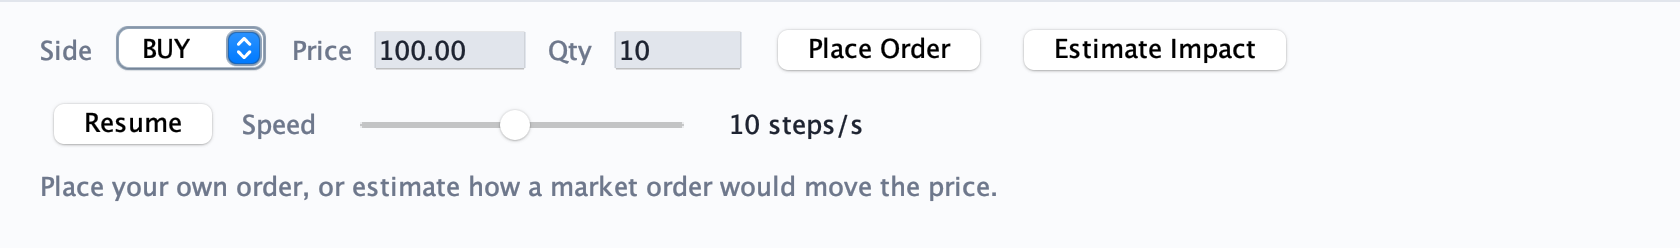
\includegraphics[width=\linewidth]{figures/fig_controls_paused.png}
\caption{Control panel while paused, with the speed set to 10 steps per second.}
\label{fig:paused}
\end{figure}

\section{Input and Output Demonstrations}

Table~\ref{tab:io} lists the actions of Section~4.2 as input--output pairs. The same cases, together with the validation cases of Section~4.4 and the engine rules (matching at the resting price, resting of the remainder, trade-log limit and a book that never crosses over 1000 simulated steps), were also executed against the real window with a small throw-away test driver; all of them produced the expected output.

\begin{table}[H]
\centering\small
\caption{Input and output of the main user actions.}
\label{tab:io}
\begin{tabular}{@{}c l r r L{6.1cm}@{}}
\toprule
\textbf{No.} & \textbf{Action} & \textbf{Price} & \textbf{Qty} & \textbf{Observed output}\\
\midrule
1 & BUY, Place Order & 101.42 & 120 & ``BUY 120 @ 101.42: 120 filled, 0 resting''; 5 trades at 100.42--101.00; best ask 100.42 $\rightarrow$ 101.00.\\
2 & BUY, Place Order & 100.23 & 40 & ``BUY 40 @ 100.23: 0 filled, 40 resting''; new bid level 100.23 with 40 units.\\
3 & BUY, Estimate Impact & -- & 300 & ``BUY 300 at market: filled=300 avg=101.02 impact=0.38''; book unchanged.\\
4 & SELL, Place Order & 85.55 & 1000 & ``SELL 1000 @ 85.55: 1000 filled, 0 resting''; best bid 100.28 $\rightarrow$ 99.66; spread 0.72 $\rightarrow$ 1.34.\\
5 & Pause, speed 10 & -- & -- & Button shows ``Resume''; label shows ``10 steps/s''; timer delay 100~ms.\\
\bottomrule
\end{tabular}
\end{table}

\section{Error Handling Demonstrations}

Figure~\ref{fig:errors} shows the message line for five invalid inputs. In every case the message is red, the book and the trade list are unchanged and the simulation keeps running. Table~\ref{tab:errors} lists these and further invalid inputs that were verified.

\begin{figure}[htbp]
\centering
\begin{subfigure}{\linewidth}
 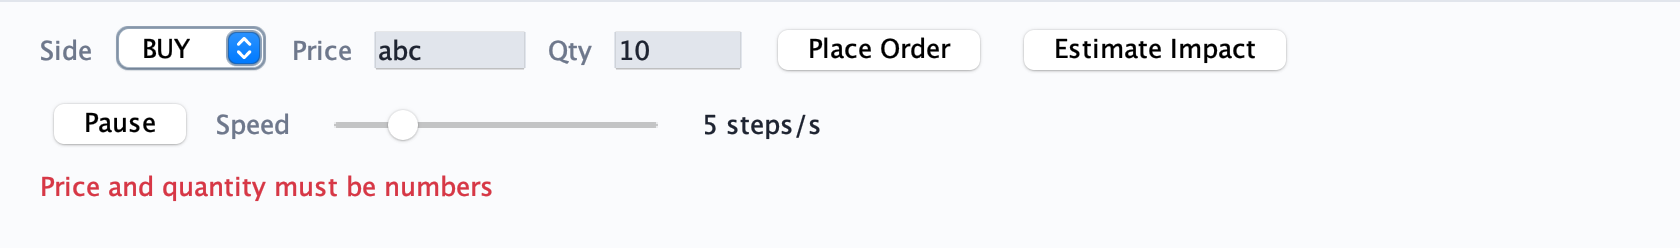
\includegraphics[width=\linewidth]{figures/err_numbers.png}
 \caption{Price \code{abc}, quantity 10.}
\end{subfigure}\par\smallskip
\begin{subfigure}{\linewidth}
 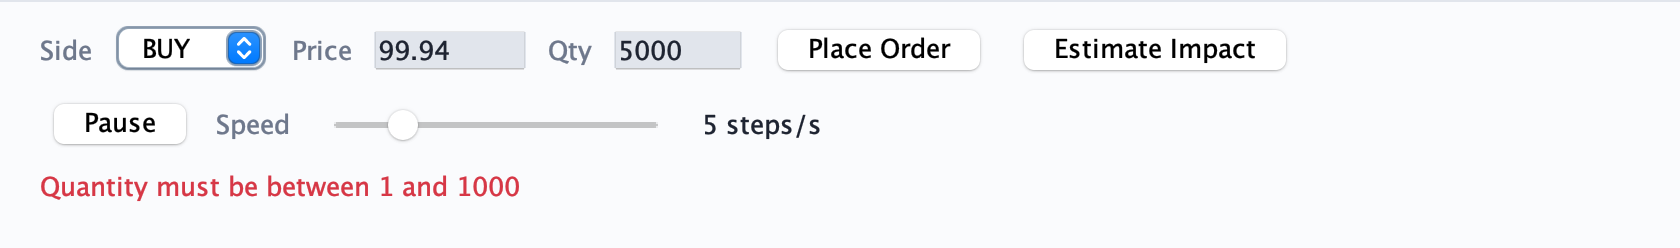
\includegraphics[width=\linewidth]{figures/err_qty.png}
 \caption{Quantity 5000.}
\end{subfigure}\par\smallskip
\begin{subfigure}{\linewidth}
 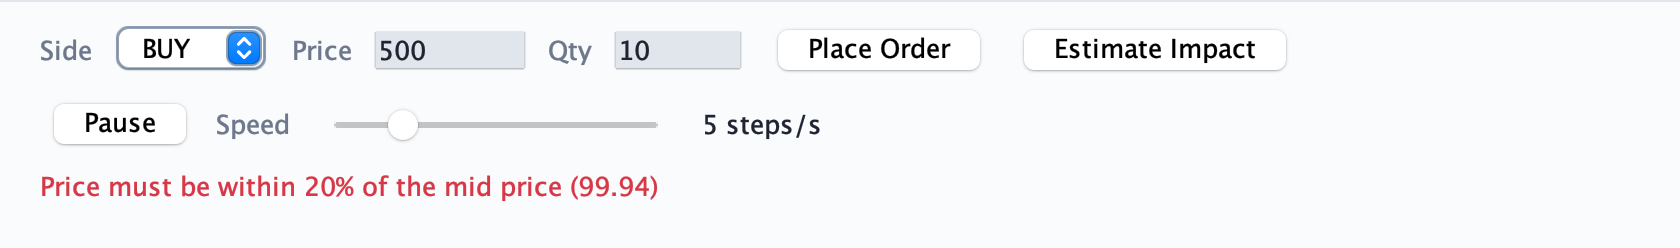
\includegraphics[width=\linewidth]{figures/err_band.png}
 \caption{Price 500 while the mid price is 99.94.}
\end{subfigure}\par\smallskip
\begin{subfigure}{\linewidth}
 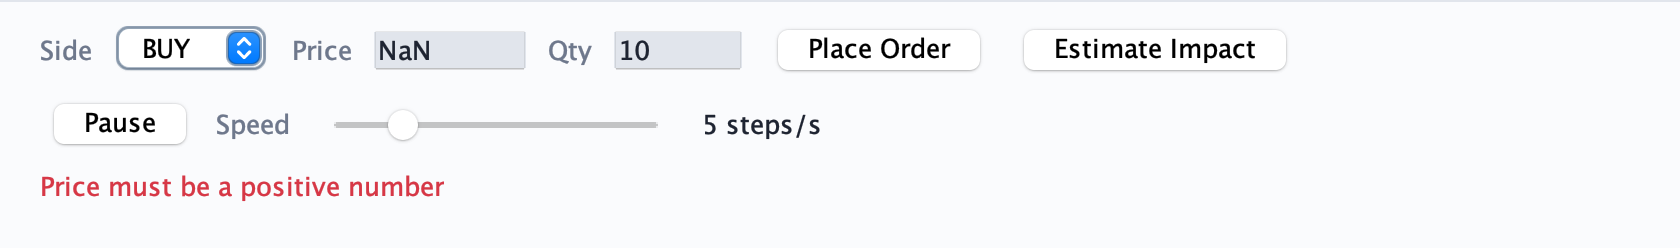
\includegraphics[width=\linewidth]{figures/err_nan.png}
 \caption{Price \code{NaN} (rejected by the \code{Order} constructor).}
\end{subfigure}\par\smallskip
\begin{subfigure}{\linewidth}
 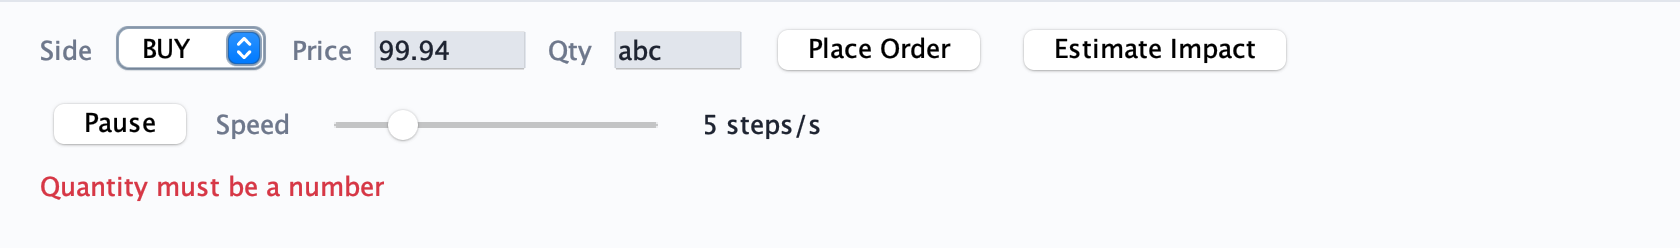
\includegraphics[width=\linewidth]{figures/err_estimate.png}
 \caption{\emph{Estimate Impact} with quantity \code{abc}.}
\end{subfigure}
\caption{Error messages for invalid input.}
\label{fig:errors}
\end{figure}

\begin{table}[H]
\centering\small
\caption{Invalid inputs and the messages produced.}
\label{tab:errors}
\begin{tabular}{@{}L{4.6cm} L{10.2cm}@{}}
\toprule
\textbf{Input} & \textbf{Message}\\
\midrule
Price empty, \code{abc} & Price and quantity must be numbers\\
Quantity empty, \code{abc}, \code{1.5} & Price and quantity must be numbers\\
Quantity \code{0}, \code{-3}, \code{1001}, \code{5000} & Quantity must be between 1 and 1000\\
Price \code{0}, \code{-5}, \code{500}, \code{Infinity} & Price must be within 20\% of the mid price (\emph{mid})\\
Price \code{NaN} & Price must be a positive number\\
Estimate Impact, quantity \code{abc} & Quantity must be a number\\
Estimate Impact, quantity \code{0} & Quantity must be between 1 and 1000\\
\bottomrule
\end{tabular}
\end{table}

\section*{Conclusion}

\projectTitle{} meets its objectives. It provides a working price-priority limit order book, a repeatable simulation of three market participants, a live view of the mid price, the depth of the book and the latest trades, and an interactive way to experiment with orders. The design is small and layered, the engine is independent of the user interface, and invalid input is reported cleanly through exceptions. The limitations listed in Section~1.4, mainly the absence of order cancellation, per-trader profit and loss and time priority within a price level, point directly to the next steps for the project.

% =====================================================================
%  REFERENCES
% =====================================================================
\renewcommand{\bibname}{References}
\clearpage
\addcontentsline{toc}{chapter}{References}
\begin{thebibliography}{99}
\setlength{\itemsep}{4pt}
\bibitem{harris2003} L.~Harris, \emph{Trading and Exchanges: Market Microstructure for Practitioners}. New York, NY, USA: Oxford University Press, 2003.
\bibitem{gould2013} M.~D. Gould, M.~A. Porter, S.~Williams, M.~McDonald, D.~J. Fenn, and S.~D. Howison, ``Limit order books,'' \emph{Quantitative Finance}, vol.~13, no.~11, pp. 1709--1742, 2013.
\bibitem{swingtutorial} Oracle, ``The Java Tutorials: Creating a GUI with Swing.'' [Online]. Available: \url{https://docs.oracle.com/javase/tutorial/uiswing/}
\bibitem{treemapapi} Oracle, ``Java Platform, Standard Edition 17 API Specification: \code{java.util.TreeMap}.'' [Online]. Available: \url{https://docs.oracle.com/en/java/javase/17/docs/api/java.base/java/util/TreeMap.html}
\bibitem{timerapi} Oracle, ``Java Platform, Standard Edition 17 API Specification: \code{javax.swing.Timer}.'' [Online]. Available: \url{https://docs.oracle.com/en/java/javase/17/docs/api/java.desktop/javax/swing/Timer.html}
\bibitem{collectionstutorial} Oracle, ``The Java Tutorials: Collections.'' [Online]. Available: \url{https://docs.oracle.com/javase/tutorial/collections/}
\bibitem{exceptionstutorial} Oracle, ``The Java Tutorials: Exceptions.'' [Online]. Available: \url{https://docs.oracle.com/javase/tutorial/essential/exceptions/}
\bibitem{effectivejava} J.~Bloch, \emph{Effective Java}, 3rd ed. Boston, MA, USA: Addison-Wesley, 2018.
\bibitem{clrs} T.~H. Cormen, C.~E. Leiserson, R.~L. Rivest, and C.~Stein, \emph{Introduction to Algorithms}, 3rd ed. Cambridge, MA, USA: MIT Press, 2009.
\end{thebibliography}

\end{document}
